%%%%%%%%%%%%%%%%%%%%%%%%%%%%%%%%%%%%%%%%%%%%%%%%%%%%%%%%%%%%
%%% LIVECOMS ARTICLE TEMPLATE FOR BEST PRACTICES GUIDE
%%% ADAPTED FROM ELIFE ARTICLE TEMPLATE (8/10/2017)
%%%%%%%%%%%%%%%%%%%%%%%%%%%%%%%%%%%%%%%%%%%%%%%%%%%%%%%%%%%%
%%% PREAMBLE
\documentclass[9pt,lessons]{livecoms}
% Use the 'onehalfspacing' option for 1.5 line spacing
% Use the 'doublespacing' option for 2.0 line spacing
% Use the 'lineno' option for adding line numbers.
% Use the "ASAPversion' option following article acceptance to add the DOI and relevant dates to the document footer.
% Use the 'pubversion' option for adding the citation and publication information to the document footer, when the LiveCoMS issue is finalized.
% The 'bestpractices' option for indicates that this is a best practices guide.
% Omit the bestpractices option to remove the marking as a LiveCoMS paper.
% Please note that these options may affect formatting.

\usepackage{lipsum} % Required to insert dummy text
\usepackage[version=4]{mhchem}
\usepackage{siunitx}
\DeclareSIUnit\Molar{M}
\usepackage[italic]{mathastext}
\graphicspath{{figures/}}
\usepackage{subfigure}
\usepackage{multirow}
%%%%%%%%%%%%%%%%%%%%%%%%%%%%%%%%%%%%%%%%%%%%%%%%%%%%%%%%%%%%
%%% IMPORTANT USER CONFIGURATION
%%%%%%%%%%%%%%%%%%%%%%%%%%%%%%%%%%%%%%%%%%%%%%%%%%%%%%%%%%%%

\newcommand{\versionnumber}{1.0}  % you should update the minor version number in preprints and major version number of submissions.
\newcommand{\githubrepository}{\url{https://github.com/DanielMarkthaler/PMF_Artifacts_LessonsLearned_LiveCoMS}}  %this should be the main github repository for this article


%%%%%%%%%%%%%%%%%%%%%%%%%%%%%%%%%%%%%%%%%%%%%%%%%%%%%%%%%%%%
%%% ARTICLE SETUP
%%%%%%%%%%%%%%%%%%%%%%%%%%%%%%%%%%%%%%%%%%%%%%%%%%%%%%%%%%%%
\title{Lessons Learned from the Calculation of One-Dimensional Potentials of Mean Force [Article v\versionnumber]}

\author[1]{Daniel Markthaler}
\author[2]{Sven Jakobtorweihen}
\author[1*]{Niels Hansen}
\affil[1]{Institute of Thermodynamics and Thermal Process Engineering, University of Stuttgart, D-70569 Stuttgart, Germany}
\affil[2]{Institute of Thermal Separation Processes, Hamburg University of Technology, D-21073 Hamburg, Germany}

\corr{hansen@itt.uni-stuttgart.de}{NH}

\orcid{Sven Jakobtorweihen}{0000-0001-5492-8304}
\orcid{Niels Hansen}{0000-0003-4366-6120}

\blurb{This LiveCoMS document is maintained online on GitHub at \githubrepository; to provide feedback, suggestions, or help improve it, please visit the GitHub repository and participate via the issue tracker.}

%%%%%%%%%%%%%%%%%%%%%%%%%%%%%%%%%%%%%%%%%%%%%%%%%%%%%%%%%%%%
%%% PUBLICATION INFORMATION
%%% Fill out these parameters when available
%%% These are used when the "pubversion" option is invoked
%%%%%%%%%%%%%%%%%%%%%%%%%%%%%%%%%%%%%%%%%%%%%%%%%%%%%%%%%%%%
\pubDOI{10.XXXX/YYYYYYY}
\pubvolume{<volume>}
\pubissue{<issue>}
\pubyear{<year>}
\articlenum{<number>}
\datereceived{Day Month Year}
\dateaccepted{Day Month Year}

%%%%%%%%%%%%%%%%%%%%%%%%%%%%%%%%%%%%%%%%%%%%%%%%%%%%%%%%%%%%
%%% ARTICLE START
%%%%%%%%%%%%%%%%%%%%%%%%%%%%%s%%%%%%%%%%%%%%%%%%%%%%%%%%%%%%%

\begin{document}

\begin{frontmatter}
\maketitle

%%%%%%%%%%%%%%%%%%%%%%%%%%%%%%%%%%%%%%%%%%%%%%%%%%%%%%%%%%%%
\begin{abstract}
%%%%%%%%%%%%%%%%%%%%%%%%%%%%%%%%%%%%%%%%%%%%%%%%%%%%%%%%%%%%

The origins of different computational artifacts that may occur in the calculation of one-dimensional potentials of mean force (PMF) from Umbrella Sampling molecular dynamics simulations and show up 
as free energy offset between bulk solvent regions are investigated.
By systematic studies, three distinct causes are elucidated:
(i) an unfortunate choice of reference points for the Umbrella distance restraint; 
(ii) a misfit in probability distributions between bound and unbound Umbrella windows in case of multiple binding modes; 
(iii) artifacts introduced by the free energy estimator. 
Starting with a fully symmetric model system consisting of methane binding to a cylindrical host, complexity is increased through the introduction of dipolar interactions between the host and the solvent, the host and the guest molecule or between all involved species, respectively. 
The manifestation of artifacts is illustrated and their origin and prevention is discussed. 
Finally, the consequences for the calculation of standard binding free enthalpies is illustrated using the complexation of primary alcohols to $\alpha$-cyclodextrin as an example.

\end{abstract}
\end{frontmatter}


%%%%%%%%%%%%%%%%%%%%%%%%%%%%%%%%%%%%%%%%%%%%%%%%%%%%%%%%%%%%
\section{Introduction}
%%%%%%%%%%%%%%%%%%%%%%%%%%%%%%%%%%%%%%%%%%%%%%%%%%%%%%%%%%%%

The field of \textit{in silico} pharmaceutical drug design impressively demonstrates  the potential of state-of-the-art free energy molecular dynamics (MD) simulations~\cite{leelananda2016computational}.
However, despite a sound theoretical basis~\cite{gilson1997statistical, boresch2003absolute} and the emergence of best practices~\cite{pohorille2010good}, 
reliable predictions of the standard binding free enthalpy for realistic host-guest systems from computer simulations are still far from routine. 
As revealed by different case studies, the discrepancy between computed and experimental estimates of the standard binding free enthalpy is often beyond the threshold of 4.2~kJ~mol$^{-1}$, 
referred to as chemical accuracy~\cite{pople1999nobel}.
Such deviations may arise from three main simulation-related sources: 
(i) the force-field problem~\cite{rocklin2013calculating,yin2015toward}, (ii) the sampling problem~\cite{zuckerman2011equilibrium} and (iii) the choice of the free-energy estimator~\cite{christ2010basic}. 
In addition, experimental uncertainties also have to be considered~\cite{van2006biomolecular} as well as incompatible thermodynamic state points~\cite{konig2012predicting} 
and artifacts caused by the simulation methods itself or wrong use of them~\cite{wong2016good}.
The present article covers two of these issues - the sampling problem and methodological artifacts.

In general, two different strategies can be utilized to compute the binding free enthalpy, related either to alchemical double decoupling, or to physical pathway methods such as potential of mean force (PMF) computations~\cite{deng2009computations}.
The latter class of methods require an integration of the PMF over a bound and unbound region, corresponding to the reversible work to transfer the ligand (or guest molecule) from the bulk to the binding pose inside the host.
In principle, the PMF-derived estimate of the binding free enthalpy can be validated by results from double decoupling~\cite{markthaler2017molecular, gumbart2012standard} or, when possible, 
by direct counting estimation, based on long unbiased simulations~\cite{pan2017quantitative, baz2018insights}.
PMF calculations for a specific binding process, are based upon either equilibrium methods such as Umbrella Sampling~\cite{torrie1974monte, torrie1977nonphysical}, Local Elevation~\cite{huber1994local}, 
Adaptive Biasing Force~\cite{darve2008adaptive}, Forward Flux Sampling~\cite{allen2009forward} or on non-equilibrium methods such as steered MD~\cite{isralewitz2001steered_1}.
In this article, we focus on one-dimensional PMFs obtained from Umbrella Sampling simulations for host molecules, featuring a distinct hydrophobic cavity.
Examples for these types of hosts range from rather low-molecular substances such as cyclodextrins~\cite{del2004cyclodextrins} or cucurbiturils~\cite{velez2012force, velez2013overcoming}, 
up to large moieties such as protein channels inside a membrane~\cite{allen2006ion, allen2006molecular, hub2010g_wham, flood2019atomistic}.
The cavity, enabling a ligand to be bound with high affinity and specificity, makes such host molecules attractive for applications in (computer-aided) drug design.
However, it also poses various challenges regarding the applied simulation protocol.
Studies of cucurbituril complexes revealed that thermodynamic irreversibilities can occur when certain guest atoms, that are not directly controlled via the bias potential, become stuck inside the host and then suddenly jump outside~\cite{velez2012force, velez2013overcoming}.
It was concluded that these dissipative conformational jumps might be a fundamental problem when applying steered MD but also Umbrella Sampling with fixed spring attachment points to flexible molecules.
In typical applications of restrained MD simulations to such molecular systems, a one-dimensional PMF is evaluated by pulling or restraining the ligand along some (linear) path from the bulk at one side of the simulation 
box through the host to the bulk at the other side.
Depending on the complexity of the system, it can be necessary to reduce the sampled space and thus to accelerate convergence by using auxiliary restraints in the simulation setup.
The concrete choice of these auxiliary restraints is however non-trivial, since a rigorous way to estimate their effect on the calculated binding free enthalpy is required in order to remove it afterwards~\cite{woo2005calculation, boresch2003absolute}.
For vanishing interactions at large distances between the binding partners, the PMF becomes flat and approaches a constant value.
The fact that this constant has to be the same for every ligand position within the bulk region (due to the isotropy of the bulk fluid in the absence of external potentials), can be used as a diagnostic test.
In a couple of published examples~\cite{filippini2012energetic, filippini2012association, allen2006ion, allen2006molecular, bacstuug2008potential, hub2010g_wham}, an artificial offset is visible in the free energy profile between the two bulk regions of the solvent which violates the state function property of the free energy.
In some of the cases, this offset was offhandedly interpreted as indication of insufficient simulation time~\cite{bacstuug2008potential}.
However, systematic studies about the origins of these artifacts are scarce~\cite{velez2013overcoming}. 
Hub et al.~\cite{hub2010g_wham} considered solute permeation across a protein channel and found that limited sampling inside the channel in the presence of locally different correlation times can lead to PMF offsets up to 15~kJ~mol$^{-1}$.
In Ref.~\citenum{allen2006ion}, such an offset was explained by accumulation of noise originating from all degrees of freedom other than the chosen order parameter, leading to a very small average force across the channel.
To remedy this problem, the authors followed similar routes: 
Ref.~\citenum{allen2006ion} proposed a symmetrization procedure by creating duplicate Umbrella windows on opposite sides of the channel, while Ref.~\citenum{hub2010g_wham} implemented a modified version of the weighted histogram analysis method (WHAM), featuring an additional constraint to enforce periodicity.
While such pragmatic solutions may suppress the occurrence of PMF offsets, they do not solve the underlying sampling problem itself.
The latter can be solved however using sampling times in excess of microseconds combined with enhanced sampling methods~\cite{sun2018molecular}.

The purpose of the present contribution is to demonstrate that computational artifacts may easily occur on much simpler systems for which advanced sampling techniques are not necessarily applied.
We elucidate various causes for PMF offsets and relate them to properties of the host-guest system and the applied simulation protocol.
The difficulty for setting up free energy molecular dynamics simulations decreased a lot over the last decades, allowing also less experienced users to obtain binding free enthalpy estimates for realistic biomolecular systems.
The critical assessment of the results including inspection for convergence and artifacts will always require advanced experience and knowledge, however.
With the systematic discussion of the reported artifacts we aim to sensitize especially newcomers and non-experts in the field in order to prevent time-consuming pitfalls in the context of binding free enthalpy calculations.

%%%%%%%%%%%%%%%%%%%%%%%%%%%%%%%%%%%%%%%%%%%%%%%%%%%%%%%%%%%%
\section{Theory}
\label{sec:theory_DG0}
%%%%%%%%%%%%%%%%%%%%%%%%%%%%%%%%%%%%%%%%%%%%%%%%%%%%%%%%%%%%

Although the main goal is to discuss PMF artifacts, for better evaluation of the results, it is advisable to calculate binding free enthalpies ($\Delta G^\circ_\mathrm{bind}$) from the PMFs.
More important, when using additional restraints on the ligand, the PMF depends on the details of these restraints but $\Delta G^\circ_\mathrm{bind}$ can be calculated by taking into account the specific restraints.
In other words, $\Delta G^\circ_\mathrm{bind}$ should be independent of the concrete choice of restraints. 
Furthermore, $\Delta G^\circ_\mathrm{bind}$ is directly related to the binding equilibrium constant and as such enables validation against experimentally determined equilibrium constants~\cite{markthaler2017molecular}.
%
A detailed derivation how to calculate $\Delta G^\circ_\mathrm{bind}$ from the PMF is beyond the scope of the current work.
Therefore, we will just outline the central ideas and present the final expressions. 
For rigorous derivations, we refer to Refs.~\citenum{deng2009computations} and \citenum{zhou2009theory}.
The link between an appropriately defined PMF and $\Delta G^\circ_\mathrm{bind}$ can be formulated as the ratio of two configurational integrals over a bound (b) and unbound (u) region: 
\begin{equation}
	\Delta G^\circ_\mathrm{bind} =  
	 -RT \ln\left(
	\frac{\int_\mathrm{b}{\mathrm{e}^{- W(\text{\boldmath $r$}_\mathrm{HL},\text{\boldmath$\omega$}_\mathrm{HL})/RT} \mathrm{d}\text{\boldmath $r$}_\mathrm{HL} \mathrm{d}\text{\boldmath$\omega$}_\mathrm{HL}}}
	{\int_\mathrm{u}{\mathrm{e}^{- W(\text{\boldmath $r$}_\mathrm{HL},\text{\boldmath$\omega$}_\mathrm{HL})/RT} \mathrm{d}\text{\boldmath $r$}_\mathrm{HL} \mathrm{d}\text{\boldmath$\omega$}_\mathrm{HL}}}
	\right) -RT \ln\left(\frac{V_\mathrm{u}}{V^\circ}\right)
	\label{eq:DG0_1}
\end{equation}
where $V^\circ = 1.661~\mathrm{nm}^3$ is the standard state volume and $R T$ is the thermal energy.
The PMF $W$ appearing in the Boltzmann factor, originally depends on the relative separation vector $\text{\boldmath $r$}_\mathrm{HL}$ and the relative orientation vector $\text{\boldmath$\omega$}_\mathrm{HL}$ 
between host and ligand. In particular, the PMF does not depend on the external degrees of freedom of the complex corresponding to the absolute position and the overall orientation inside the simulation box.
The second term  accounts for the free energy contribution of the volume change from the standard state volume $V^\circ$ to the unbound volume $V_\mathrm{u}$. 
It should be noted that $V_\mathrm{u}$, which depends on the size of the simulation box cancels from the final expression for $\Delta G^\circ_\mathrm{bind}$~\cite{general2010note}.
Depending upon the choice of coordinates, a Jacobian determinant may arise in the configurational integrals of Eq.~(\ref{eq:DG0_1}), which has been omitted for brevity however.

Due to the complexity of the systems, it is often necessary to use auxiliary restraints in the simulation setup. 
The effect of such additional restraints that limit the phase space to be sampled during the transfer of the ligand from the standard state volume to the binding pose of the host, 
can be incorporated by introduction of intermediate states into Eq.~(\ref{eq:DG0_1})~\cite{woo2005calculation}.
The approach can be visualized in the form of a thermodynamic cycle as depicted in Fig.~\ref{fig:thermo_cycle}.
\begin{figure}[htb!]
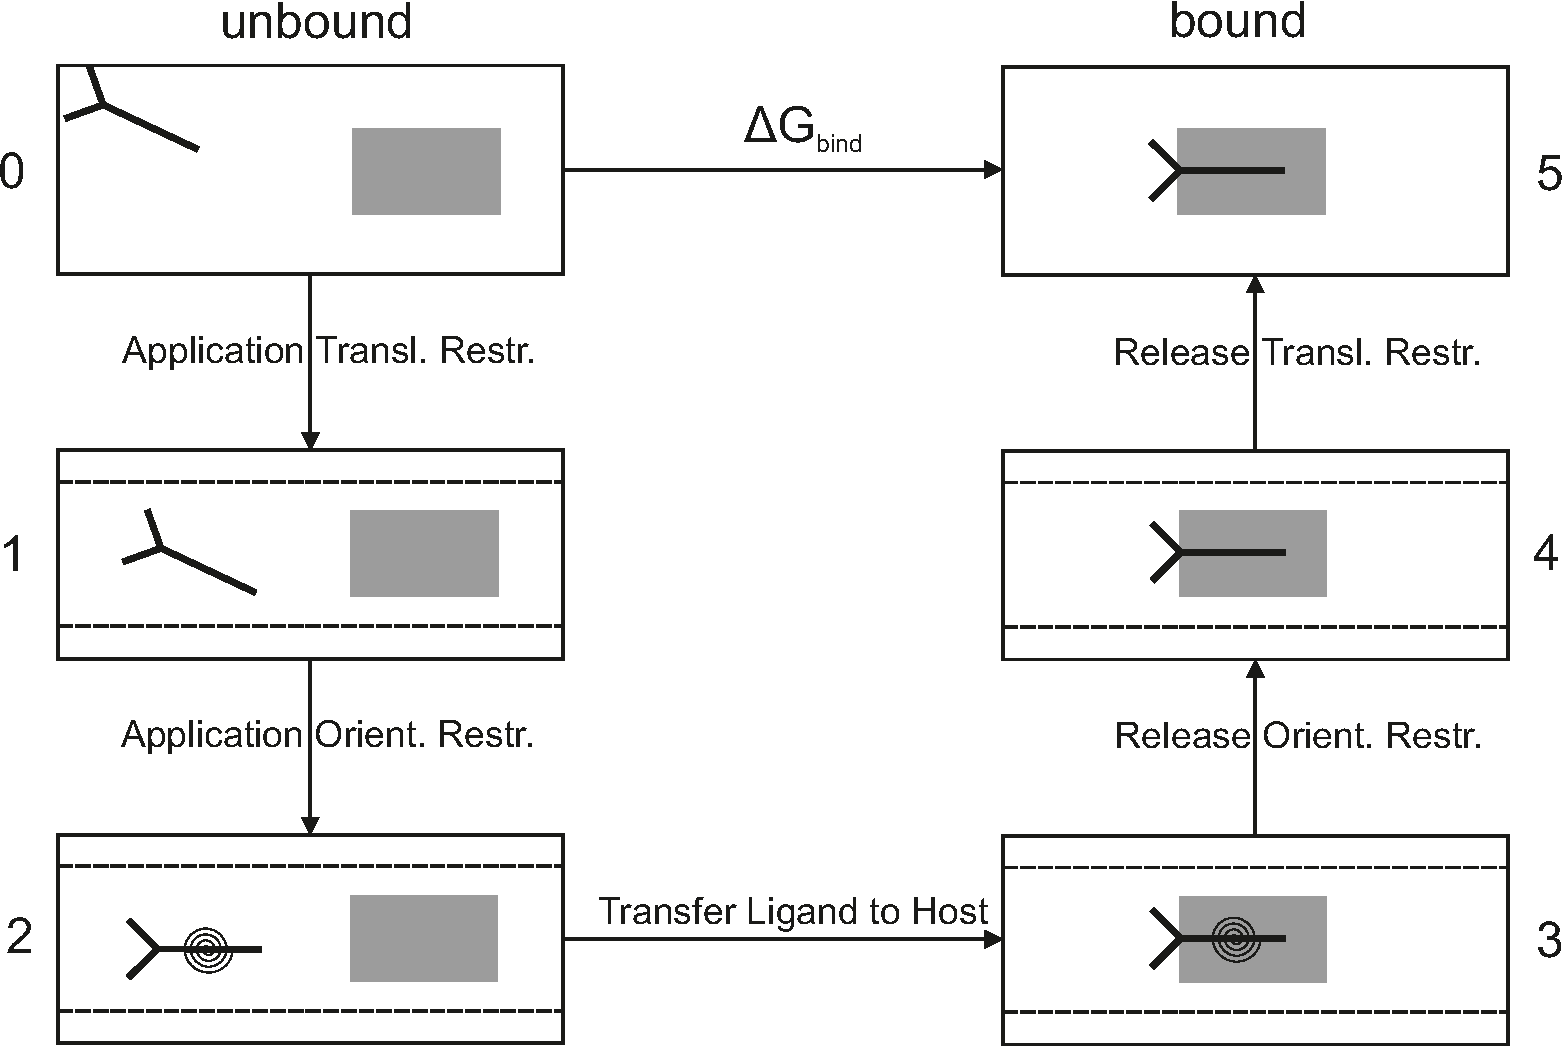
\includegraphics[width=\linewidth]{figures/thermocycle.pdf}
\caption{Thermodynamic cycle for the calculation of the binding free enthalpy $\Delta G_\mathrm{bind}$.
The host and ligand molecule are represented by the grey rectangle and black structure, respectively.
The free enthalpy difference between the unbound (point 0) and bound (point 5) state is given by $\Delta G_\mathrm{bind}$. 
When the volume in point 0 is given by  the standard state volume $V^\circ$, $\Delta G_\mathrm{bind}$ corresponds to the standard binding free enthalpy $\Delta G^\circ_\mathrm{bind}$.
Due to the path-independence of $\Delta G_\mathrm{bind}$, it can be calculated not only from the direct path $0 \rightarrow 5$ as accessed experimentally but equivalently from an indirect path such as 
$0 \rightarrow 1  \rightarrow 2  \rightarrow 3  \rightarrow 4  \rightarrow 5$ as accessed from molecular simulations, including several intermediate states (see main text).
}
\label{fig:thermo_cycle}
\end{figure}

Application to the case of a PMF along a one-dimensional order parameter ($\zeta$) including auxiliary translational and orientational restraints on the ligand (c.f. Sec.~\ref{sec:theory_setup}), 
finally yields the following expression for $\Delta G^\circ_\mathrm{bind}$~\cite{markthaler2017molecular, doudou2009standard}: 
\begin{equation}
\Delta G^\circ_\mathrm{bind} = \Delta G_\mathrm{V} + \Delta G_\Omega + \Delta W_\mathrm{R} + \Delta G_\theta + \Delta G_\rho
\label{eq:DG0_2}
\end{equation}
%
with terms ordered according to the cycle in Fig.~\ref{fig:thermo_cycle}:
\begin{eqnarray*}
\Delta G_\mathrm{V} & = &  - RT \ln\left(\frac{l_\mathrm{b} A_{\mathrm{u},\rho}}{V^\circ}\right) \\
\Delta G_\Omega & = & - RT \ln\left(\frac{\Omega}{8 \pi^2}\right) \\
\Delta G_\theta & = & RT \ln\left(\langle  \mathrm{e}^{- U_\theta(\theta)/RT}  \rangle_{\mathrm{b}, k_\theta=0}\right) \\
\Delta G_\rho & = & RT \ln\left(\langle  \mathrm{e}^{- U_\rho(\rho)/RT}  \rangle_{\mathrm{b}, k_\rho=0}\right)
\end{eqnarray*}
$\Delta W_\mathrm{R}$ denotes the depth of the one-dimensional PMF $W_\mathrm{R}(\zeta)$ towards its global minimum where the guest molecule is bound.
When the global PMF minimum is defined to be zero as it was done in this work, $\Delta W_\mathrm{R}$ corresponds to the negative PMF value in the bulk ($W_{\mathrm{R},\infty}$): 
$\Delta W_\mathrm{R} = - W_{\mathrm{R},\infty}$.
The index "R" indicates that the PMF was evaluated in the presence of auxiliary restraints such as the orthogonal translational and orientational restraints (c.f. Sec.~\ref{sec:theory_setup}).
That is, $\Delta W_\mathrm{R}$ represents the step $2 \rightarrow 3$ in Fig.~\ref{fig:thermo_cycle}.
The integration of the PMF over the bound region, is captured in the definition of the bound length $l_\mathrm{b}$:
\begin{equation}
	l_\mathrm{b} = \int_\mathrm{b}{ \mathrm{e}^{- W_\mathrm{R}(\zeta)/RT} \mathrm{d} \zeta }
\label{eq:lb}
\end{equation}
Due to the Boltzmann-weighting in Eq.~(\ref{eq:lb}), the lowest values of $W_\mathrm{R}(\zeta)$ contribute the most to the integral while larger values at increasing distances from the minimum have smaller weights.
This makes the estimate of $l_\mathrm{b}$ and thus $\Delta G^\circ_\mathrm{bind}$ insensitive to the actual choice of the cut-off distance between bound and unbound region, in particular for rather tight binding situations as studied in the present work~\cite{gilson1997statistical}.
Here, the entire range of $\zeta$-values between the flat parts of the PMF on both sides relative to the minimum were considered as the bound region. 
The free energy contribution due to the volume change from the standard state volume $V^\circ$ to $l_\mathrm{b} \, A_{\mathrm{u},\rho}$ is described by the term $\Delta G_\mathrm{V}$ in Eq.~(\ref{eq:DG0_2}), 
corresponding to the step $0 \rightarrow 1$ in Fig.~\ref{fig:thermo_cycle}.
Therein, $A_{\mathrm{u},\rho}$ denotes the cross-sectional area which is accessible to the unbound ligand in orthogonal directions in the presence of the applied translational restraint.
Its value can be calculated analytically from the partition function of the restraining potential $U_\rho(\rho)$ used for restricting the lateral movement of the ligand in the bulk solvent~\cite{doudou2009standard, markthaler2017molecular}:
\begin{equation}
	A_{\mathrm{u},\rho} = \int\limits_{0}^\infty \mathrm{e}^{- U_\rho(\rho)/RT} \, 2 \pi \rho\, \mathrm{d}\rho
\label{eq:Au}
\end{equation}
where $\rho$ is the orthogonal distance (c.f. Fig.~\ref{fig:host_guest_sketch}). 
The term $\Delta G_\rho$ accounts for the free energy contribution of releasing the orthogonal translational restraint in the bound state ($4 \rightarrow 5$ in Fig.~\ref{fig:thermo_cycle}).
As indicated by the notation $\langle ... \rangle_{\mathrm{b}, k_\rho=0}$, this contribution may be evaluated numerically by free energy perturbation~\cite{zwanzig1954high} using exponential averaging from an additional simulation with the bound ligand at vanishing restraining force constant $k_\rho=0$~\cite{doudou2009standard}.
A more sophisticated way would be to perform the estimation within multiple simulations of decreasing values of $k_\rho$ using thermodynamic integration~\cite{kirkwood1935statistical} or the Multistate Bennett's Acceptance Ratio (MBAR) estimator~\cite{shirts2008statistically}.
%
The terms $\Delta G_\Omega$ and $\Delta G_\theta$ in Eq.~(\ref{eq:DG0_2}) assess the free energy contributions from applying and releasing the angular restraint $U_\theta$ in the unbound and bound state, respectively 
($1 \rightarrow 2$ and $3 \rightarrow 4$ in Fig.~\ref{fig:thermo_cycle}).
$\Omega$ denotes the rotational volume available to the ligand in the bulk under the influence of the angular restraint. 
For a given functional form of the restraining potential $U_\theta$, its value can be evaluated from a three-dimensional integral over the Euler angles~\cite{hermans1997inclusion, steinberg1963entropy}:
\begin{equation}
\Omega = \int\limits_{0}^{2 \pi}\int\limits_{0}^{2 \pi}\int\limits_{0}^{\pi} \mathrm{e}^{- U_\theta(\theta)/RT} \, \sin\theta \, \mathrm{d}\theta \mathrm{d}\phi \mathrm{d}\psi
              = 4 \pi^2  \int\limits_{0}^{\pi} \mathrm{e}^{- U_\theta(\theta)/RT} \, \sin\theta \, \mathrm{d}\theta
\label{eq:Omega}
\end{equation}
Depending on the functional form of $U_\theta$, this integral may be solved analytically or numerically.
If no angular restraint was applied, allowing the ligand to rotate freely in the bulk, $\Omega$ equals $8 \pi^2$ and Eq.~(\ref{eq:DG0_2}) becomes identical to Eq.~(11) of Ref.~\citenum{doudou2009standard}. 
Therein, it is assumed that the change in rotational entropy for the bound ligand is included in $\Delta W_\mathrm{R}$.
In the following we will study situations in which this assumption does not hold.
The free energy term $\Delta G_\theta$ has to be evaluated numerically by free energy perturbation or thermodynamic integration for example.

Application of standard error propagation rules to all involved quantities associated with an uncertainty in Eq.~(\ref{eq:DG0_2}) gives:
\begin{equation}
\begin{split}
\sigma^2 \left\{\Delta G^\circ_\mathrm{bind} \right\}  & = \left(  \frac{RT}{l_\mathrm{b} } \right)^2 \sigma^2 \left \{ l_\mathrm{b} \right \} + \sigma^2 \left\{ \Delta G_\Omega \right\} + \sigma^2 \left \{ \Delta W_\mathrm{R} \right \} \\\
& + \sigma^2 \left\{ \Delta G_\theta \right\} + \sigma^2 \left\{ \Delta G_\rho \right\} 
\end{split}
\label{eq:DG0_error_1}
\end{equation}
where $\sigma^2 \{...\}$ denotes the variance. 
The uncertainty in $\Delta G_\Omega$ arises from the numerical integration error associated with the applied quadrature scheme and is redundant if an analytical calculation is possible. 
Considering only the leading term in Eq.~(\ref{eq:DG0_error_1}) which is given by $\sigma^2 \left \{ \Delta W_\mathrm{R} \right \}$ and delivered by the applied estimator (c.f. Sec.~\ref{sec:estimators})  
yields the following simplified expression for the uncertainty estimate of $\Delta G^\circ_\mathrm{bind}$:
\begin{equation}
\sigma^2 \left\{\Delta G^\circ_\mathrm{bind} \right\}  \approx \sigma^2 \left \{ \Delta W_\mathrm{R} \right \}
\label{eq:DG0_error_2}
\end{equation}

%%%%%%%%%%%%%%%%%%%%%%%%%%%%%%%%%%%%%%%%%%%%%%%%%%%%%%%%%%%%
\section{Methods}
%%%%%%%%%%%%%%%%%%%%%%%%%%%%%%%%%%%%%%%%%%%%%%%%%%%%%%%%%%%%

\subsection{Host-Guest Systems}

The search for suitable host-guest benchmarks which are simple enough to approach accurately by MD simulations within reasonable time scales 
yet complex enough to feature properties of protein-ligand systems is an ongoing and non-trivial problem~\cite{mobley2017predicting}.
The majority of simulations from the current work were based on a short carbon nanotube (CNT) host without partial charges (c.f. Fig.~\ref{fig:systems}).
This model system, featuring a hydrophobic, water-free cavity resembles the situation of an ideally symmetric and unpolar host molecule. 
On the other hand, it allows the effect of molecular "asymmetries" to be studied systematically.
Here, such an asymmetry was introduced by distributing charge pairs on the terminal C-H atoms at one side of the CNT.
The investigated ligands comprised united-atom models for methane, (elongated) ethane and hexane.
The effect of dipolar ligands was modeled by placing a positive and neutralizing negative charge onto covalently bound neighboring carbon atoms in case of polyatomic ligands.
To test the validity and transferability of the protocol in case of more realistic systems, it was applied to $\alpha$-cyclodextrin ($\alpha$CD, c.f. Fig.~\ref{fig:systems}) as a host molecule of practical relevance, complexed with primary alcohols.

\begin{figure}[htb!]
  \centering    
  \subfigure[]{\label{fig:a}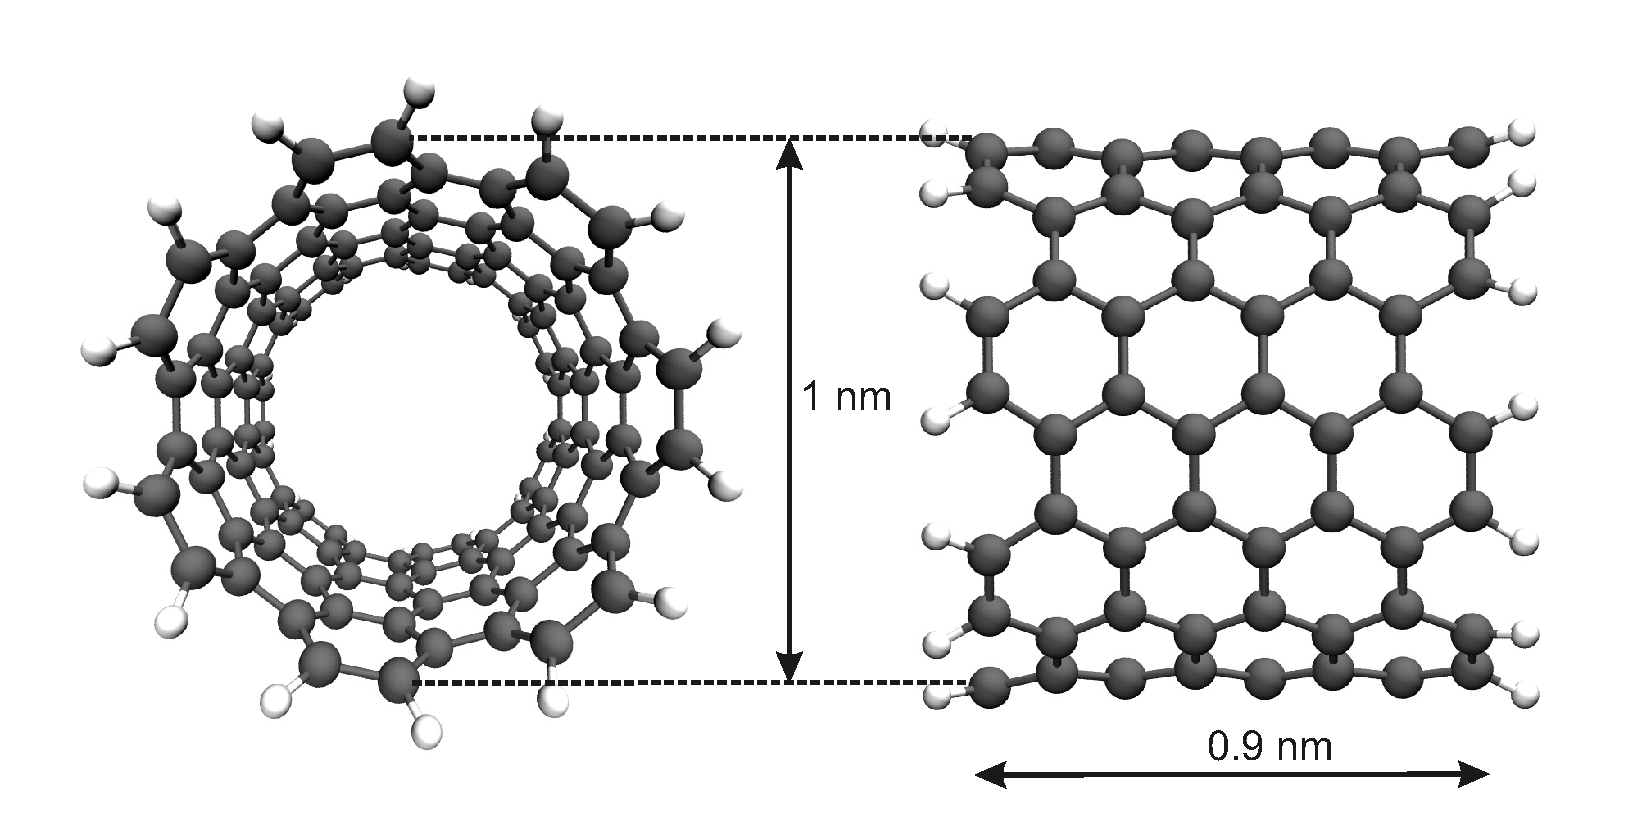
\includegraphics[width=\linewidth]{figures/CNT_system.pdf}}
  \subfigure[]{\label{fig:b}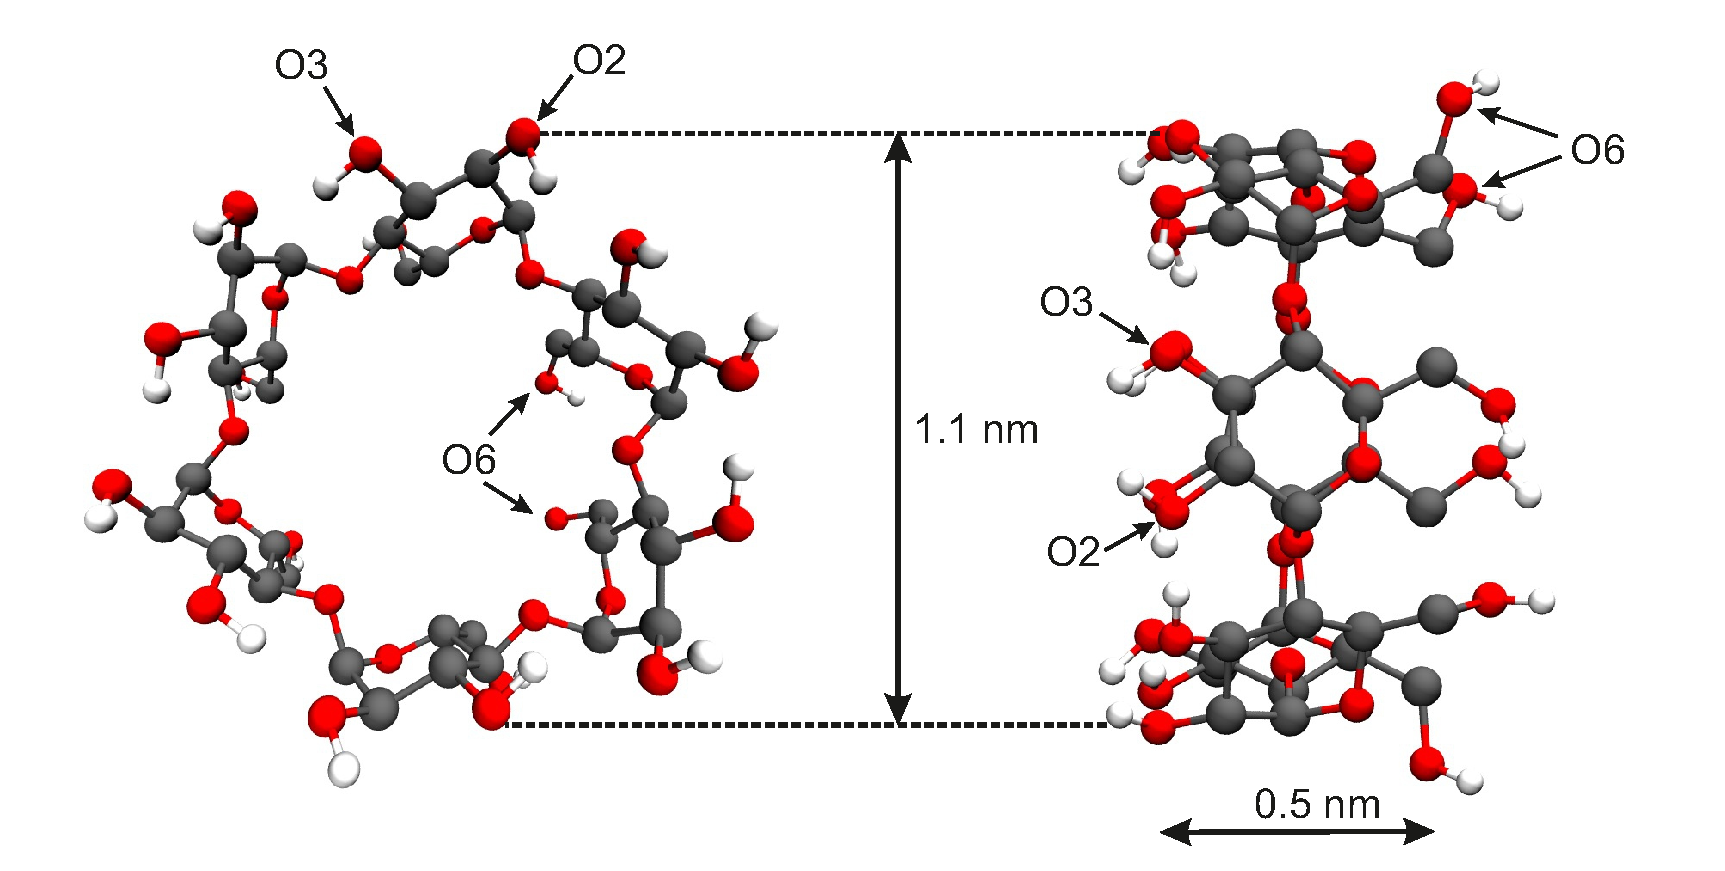
\includegraphics[width=\linewidth]{figures/aCD_system.pdf}}
  \caption{
  Carbon nanotube (CNT) model host (a) and $\alpha$-cyclodextrin ($\alpha$CD) molecule (b). The CNT is (7,7) tube in armchair structure.
  Nomenclature of $\alpha$CD-oxygen types according to Ref.~\citenum{iupac1983symbols}.
  Host dimensions are depicted in front (left) and side view (right).}
  \label{fig:systems}
\end{figure}


\subsection{Simulation Protocol}
\label{sec:theory_setup}

The PMFs were constructed from the time series of a single order parameter sampled via Umbrella Sampling~\cite{torrie1974monte, torrie1977nonphysical}, similar to the approach proposed by Doudou et al.~\cite{doudou2009standard}.
As illustrated in Fig.~\ref{fig:host_guest_sketch}, the order parameter ($\zeta$) used primarily in this work is given by the projection of the instantaneous separation vector 
($\text{\boldmath $r$}_\mathrm{HL}$) between the centers of mass (COM) of the binding partners onto the host's instantaneous symmetry axis ($\text{\boldmath$\omega$}_\mathrm{H}$):
$\zeta \equiv \text{\boldmath $r$}_\mathrm{HL} \cdot \text{\boldmath$\omega$}_\mathrm{H} = r_\mathrm{HL} \cos{\varphi}$. 
Here, the unity vector $\text{\boldmath$\omega$}_\mathrm{H}$ was defined by the connecting line through the geometric centers at both sides of the CNT.
$\varphi$ denotes the angle between $\text{\boldmath$\omega$}_\mathrm{H}$ and $\text{\boldmath $r$}_\mathrm{HL}$.
Instead of the centers of mass, two other characteristic reference points of the host and ligand could be used instead (c.f. Sec.~\ref{subsec:refpoints}).
The usage of the COM-COM radial distance ($r_\mathrm{HL} = |\text{\boldmath $r$}_\mathrm{HL}|$) itself as order parameter would lead to to artifacts around $\zeta = 0 $~\cite{you2019potential}.
It would further require the addition of a Jacobian term  $RT \ln{J(r_\mathrm{HL})}$ to the "raw" PMF estimate with Jacobian determinant $J(r_\mathrm{HL}) = 4 \pi \, r_\mathrm{HL}^2$,  
in order to obtain a constant value in the bulk at large distances~\cite{trzesniak2007comparison}.
Such a Jacobian term, which is of pure entropic nature and accounts for the increase in the accessible configurational area at increasing distances, does not arise when $\zeta$ is used instead~\cite{doudou2009standard}.
Lateral movement of the ligand at every Umbrella window was restricted with the aid of a flat-bottom potential acting on the orthogonal displacement ($\rho = r_\mathrm{HL} \sin{\varphi}$, c.f. Fig.~\ref{fig:host_guest_sketch}) 
of the ligand's COM from the host's molecular axis:
\begin{equation}
U_\rho(\rho) = \left\{\begin{array}{ll} 
		k_\rho (\rho-\rho_\mathrm{up})^n, & \mathrm{if} \, \rho > \rho_\mathrm{up} \\
		0, & \mathrm{otherwise}
		\end{array}\right. 
\label{eq:ort_restr}
\end{equation}
The flat-bottom potential (harmonic ($n = 2$) or quartic ($n = 4$), force constant $k_\rho$) is activated only when the actual displacement exceeds a certain threshold $\rho_\mathrm{up}$.
%
In this case, calculation of $A_{\mathrm{u},\rho}$ according to Eq.~(\ref{eq:Au}) yields~\cite{markthaler2017molecular}:
\begin{equation}
A_{\mathrm{u},\rho}  
		= \pi \rho_\mathrm{up}^2 +
		\left\{\begin{array}{ll} 
		\frac{2 \pi}{k_\rho^{*}} + \pi \rho_\mathrm{up} \frac{(2 \pi)^{0.5}}{k_\rho^{* 0.5}}, & \mathrm{if} \, n = 2 \\
		\frac{\pi^{1.5}}{2\, k_\rho^{* 0.5}} + \pi \rho_\mathrm{up} \frac{\Gamma(0.25)}{2\, k_\rho^{* 0.25}}, & \mathrm{if} \, n = 4
		\end{array}\right. 
\label{eq:Au_2}
\end{equation}
with the reduced restraining force constant $k_\rho^{*} \equiv k_\rho/RT$ and the Gamma function $\Gamma$.
%
If the threshold value $\rho_\mathrm{up}$ for the flat-bottom potential is chosen to be large enough compared to the size of the host's cavity 
such that the ligand's dynamic is not affected in the bound state, the term $\Delta G_\rho$ in Eq.~(\ref{eq:DG0_2}) becomes redundant.
It should be stressed that while the PMF itself and the terms $\Delta W_\mathrm{R}, \Delta G_\mathrm{V}, \Delta G_\rho$ in Eq.~(\ref{eq:DG0_2}) are influenced by the restraining parameters 
$n$, $k_\rho$ and $\rho_\mathrm{up}$, the estimate for $\Delta G^\circ_\mathrm{bind}$ should be independent when all contributions are evaluated adequately (c.f. Sec.~\ref{res:UnpMet_UnpCNT}).
%
Major modifications compared to the original approach of Doudou et al.~\cite{doudou2009standard} can be summarized as follows:
(i) the order parameters used for both, the actual PMF calculation and for measuring the ligand's orthogonal movement, are defined in a relative manner between ligand and host. 
Instead of using a particular Cartesian component such as the $z$-component of the COM-COM separation vector $\text{\boldmath $r$}_\mathrm{HL}$ with respect to an arbitrary external lab-frame coordinate system, 
we look at projections of $\text{\boldmath $r$}_\mathrm{HL}$ onto axes of a body-fixed coordinate system which is centered inside the host.
The usage of relative order parameters relaxes the requirement of a translationally and/or rotationally restrained host and allows the same approach to be used in case of a fully mobile host molecule without further modifications (c.f. Sec.~\ref{subsec:rest_host});
(ii) for the majority of ligands, an additional angular or orientational restraint in the form of a harmonic potential 
\begin{equation}
U_\theta(\theta) = \frac{k_\theta}{2}(\theta-\theta_0)^2
\label{eq:ori_restr}
\end{equation}
was applied, acting on the angle ($\theta$) between the molecular axes of host ($\text{\boldmath$\omega$}_\mathrm{H}$) and 
ligand ($\text{\boldmath$\omega$}_\mathrm{L}$) in order to suppress flipping of the ligand relative to the host.
The molecular axis of the ligand, expressed as unity vector $\text{\boldmath$\omega$}_\mathrm{L}$, was defined by the connecting line through two peripheric atoms of the ligand.
The value of $k_\theta$ should be chosen high enough to prevent transitions between different ligand orientations. 
As in case of the translational restraint, the estimate for $\Delta G^\circ_\mathrm{bind}$ should be independent of the concrete choice of $k_\theta$.
In case of a translationally and rotationally restrained host aligned along the $z$-axis of the lab frame coordinate system of the simulation box without orientational restraint on the ligand, the approach corresponds to the original setup described in Ref.~\citenum{doudou2009standard}.
In this case, the order parameter $\zeta$ corresponds to the Cartesian $z$-component of $\text{\boldmath $r$}_\mathrm{HL}$ and $\rho$ becomes $\rho = \sqrt{\Delta x^2 + \Delta y^2}$.
Here, $\Delta x$ and $\Delta y$ denote the orthogonal displacements of the ligand's COM from the central $z$-axis.

The free energy contributions corresponding to the release of the translational and orientational restraint in the bound state ($\Delta G_\rho$ and $\Delta G_\theta$ in Eq.~(\ref{eq:DG0_2})) 
were each calculated from a sequence of 20 simulations with the bound ligand located at the PMF minimum. 
The individual simulations were conducted at different scaled force constants $k_\rho(\lambda) = \lambda \cdot k_\rho$ with the scaling parameter $\lambda$ equally distributed between 0 and 1 (analogously for $k_\theta$).  
The endpoints correspond to the unrestrained case at $\lambda = 0$ and the actual force constant value as used for Umbrella Sampling at $\lambda = 1$, respectively.
Using the configurations sampled from a particular state $\lambda_\mathrm{i}$, all possible pairwise potential energy differences $\Delta_\mathrm{ij} U = U_\rho(\lambda_\mathrm{j}) - U_\rho(\lambda_\mathrm{i})$ 
towards the reference state potential $U_\rho(\lambda_\mathrm{i})$ were evaluated (analogously for $U_\theta$). 
From these potential energy differences, the free energy calculation was performed via the MBAR estimator. 
For enhanced sampling, Hamiltonian Replica Exchange between neighboring $\lambda$-points was applied with attempted exchanges every 1000 steps. 

Initial configurations for the production simulations of each Umbrella window were generated within a prior equilibration phase (500~ps per window) in the following manner:
starting in the bulk at one side of the CNT, the ligand was sequentially displaced in 0.1~nm increments 
along a linear path trough the cavity, until the unbound ligand was located in the bulk again, relative to the other side of the CNT.
For production, all considered systems were simulated at least for 20~ns per window until converged PMF estimates were obtained.
Specifications regarding the applied restraints in the protocol are summarized in Tab.~\ref{tbl:restr_1}.

\begin{figure}[htb!]
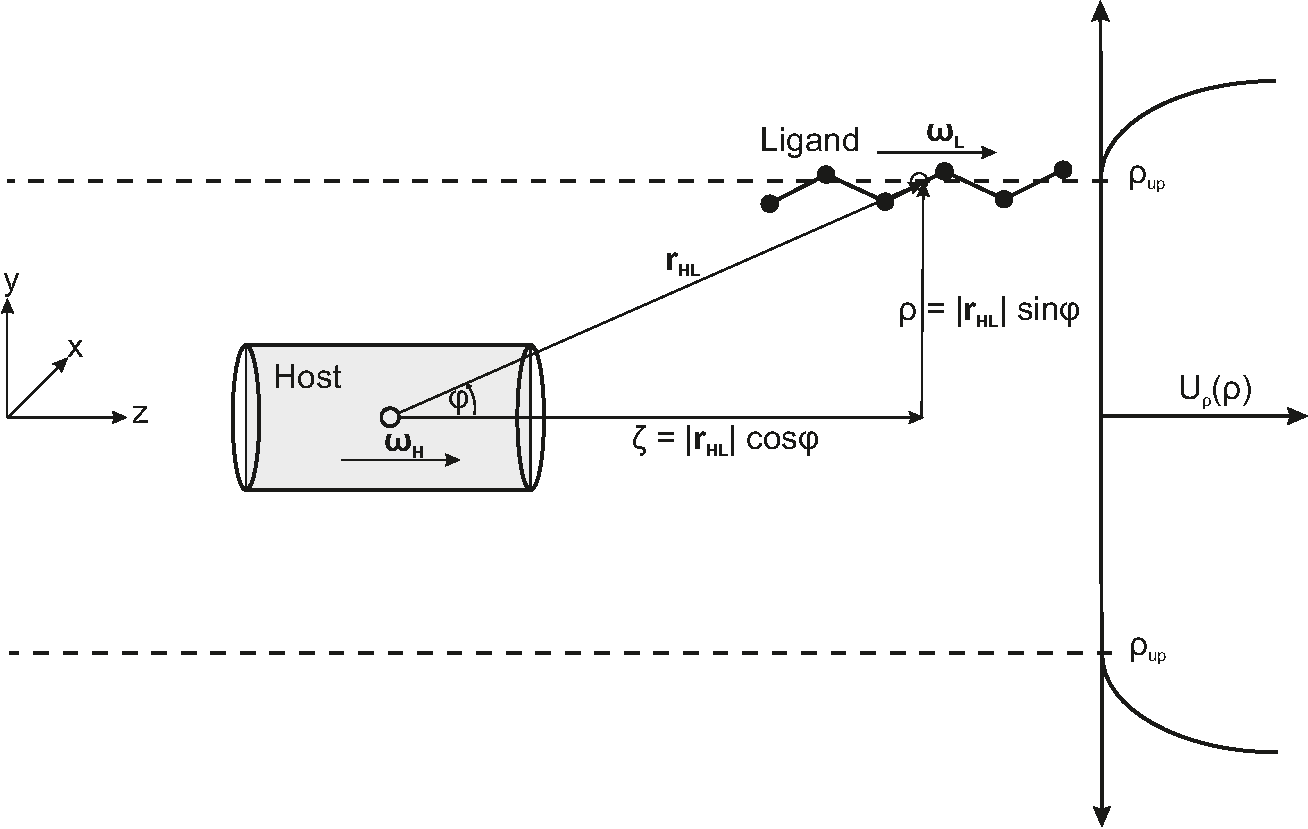
\includegraphics[width=\linewidth]{figures/sketch_simulation_protocol.pdf}
\caption{Schematic representation of the host-guest system and the relevant collective variables. 
The orientation of the ligand ($\text{\boldmath$\omega$}_\mathrm{L}$) may be aligned towards the orientation of the host ($\text{\boldmath$\omega$}_\mathrm{H}$) by the usage of an orientational restraint 
acting on the angle $\theta$ between between $\text{\boldmath$\omega$}_\mathrm{L}$ and $\text{\boldmath$\omega$}_\mathrm{H}$ (see main text).
$\varphi$ denotes the angle between $\text{\boldmath$\omega$}_\mathrm{H}$ and the separation vector between the centers of mass of host and ligand ($\bf{r}_\mathrm{HL}$). 
The chosen order parameter ($\zeta$) is the projection of $\bf{r}_\mathrm{HL}$ onto the host's molecular axis $\text{\boldmath$\omega$}_\mathrm{H}$.
When the host itself is aligned along the $z$-axis of the lab frame coordinate system, as depicted here, the order parameter corresponds to the Cartesian $z$-component of $\bf{r}_\mathrm{HL}$. %, denoted as $z$. 
The ligand's movement orthogonal to the order parameter outside the host, is restricted by a  flat-bottom potential ($U_\rho(\rho)$) acting on the orthogonal distance ($\rho$) 
between the center of mass of the ligand and the molecular axis of the host. 
The flat-bottom potential is activated when the actual distance $\rho$ exceeds a certain threshold distance ($\rho_\mathrm{up}$), as depicted by the dashed lines.}
\label{fig:host_guest_sketch}
\end{figure}

\begin{table}[ht]
\caption{\label{tbl:restr_1}
Default values for restraints specifying the Umbrella Sampling protocol as used for the majority of studies in the current work. 
In case of differing settings, the parameter choice is explicitly given.
For all simulations involving a polar CNT, a value of $k_\zeta = 3000~\mathrm{kJ~mol^{-1}~nm^{-2}}$ was used for the distance restraint force constant. 
Lateral translational movement of the ligand (as measured by the orthogonal displacement $\rho$) was restrained using a flat-bottom potential (c.f. Eq.~(\ref{eq:ort_restr})).
To restrain the ligand's orientation towards a specific bound state orientation, an orientational restraint acting on the angle $\theta$ between the molecular axes of host and ligand was applied (c.f. Eq.~(\ref{eq:ori_restr})). 
}
\centering
\begin{tabular}{cccc}\hline
\multicolumn{4}{c}{Distance Restraint} \\\hline
$k_\zeta$ & $\zeta_\mathrm{min}$ & $\zeta_\mathrm{max}$ & $\Delta \zeta$ \\
$[\mathrm{kJ~mol}^{-1}~\mathrm{nm}^{-2}]$ & $[\mathrm{nm}]$ & $[\mathrm{nm}]$ & $[\mathrm{nm}]$ \\ 
\hline
500 & -2.5 & 2.5 & 0.1 \\\hline\hline
\multicolumn{4}{c}{Translational Restraint}  \\\hline
$k_\rho$ & $\rho_\mathrm{up}$ & $n$ \\
$[\mathrm{kJ~mol}^{-1}~\mathrm{nm}^{-n}]$ & $[\mathrm{nm}]$ & $[-]$ \\ 
\hline 
500 & 0.4 & 2 \\\hline\hline
\multicolumn{4}{c}{Orientational Restraint}  \\\hline
$k_\theta$ & $\theta_0$ \\
$[\mathrm{kJ~mol}^{-1}~\mathrm{rad}^{-2}]$ & $[\mathrm{rad}]$  \\ 
\hline
500 & 0.0 \\\hline
\end{tabular}
\end{table}


\subsection{Simulation Code and Parameters}
\label{sec:simparam}

The GROMOS biomolecular force field was applied throughout this work using the 54A7~\cite{schmid2011definition} and 53A6$_\mathrm{GLYC}$~\cite{pol2012gromos} parameter sets for studies based on the CNT and 
$\alpha$CD, respectively. 
The standard atom types 12 and 20 were used to represent the CNT carbon and hydrogen atoms, respectively. 
All systems were solvated in water based on the three-site simple point charge (SPC) water model~\cite{berendsen1981interaction}.
Simulations were conducted under periodic boundary conditions using the leapfrog algorithm~\cite{eastwood1981computer} for integrating Newton's equations of motion with a time step of 2~fs.
The majority of simulations were performed with the GROMACS 2016.4 program package~\cite{berendsen1995gromacs, hess2008gromacs, abraham2015gromacs}.
In the light of recent publications reporting on the sensitivity of simulation results on the choice of the pairlist algorithm, the electrostatics treatment, the cut-off scheme or other 
technical details~\cite{silva2018impact, gonccalves2019influence, reisser2017real, loeffler2018reproducibility}, complementary simulations were conducted with the GROMOS11 program package (release version 1.5.0)~\cite{kunz2012new, riniker2011calculation, schmid2012architecture} which has different recommended settings.
In particular, GROMOS is usually used with a reaction field scheme for treating long-range electrostatic interactions. Since this approach is also used by other codes in the context of free energy 
simulations~\cite{papadourakis2018blinded, aaqvist2017cold}, it is interesting to study the effect on a PMF calculation.
In the following, separated computational details are given for the two simulation codes.

\subsubsection*{GROMACS Simulations}

Simulations using the particle-mesh Ewald (PME) method~\cite{darden1993particle, essmann1995smooth} for treating electrostatic interactions were conducted with the 
GROMACS 2016.4 program~\cite{berendsen1995gromacs, hess2008gromacs, abraham2015gromacs} patched to the free-energy library 
PLUMED 2.4.2~\cite{tribello2014plumed} for restraints definition and biasing selected collective variables.
The center of mass translation of the computational box was removed every 1000~steps. 
All bond lengths were constrained using the LINCS algorithm~\cite{hess1997lincs, hess2008p} with a LINCS-order of 4. 
The number of iterations to correct for rotational lengthening in LINCS was set to 2.
SPC water was constrained using the SETTLE algorithm~\cite{miyamoto1992settle}.
Equilibration of solvated energy-minimized systems was performed within a prior 100~ps constant-volume simulation at reference temperature of 300~K, followed by a 1~ns constant-pressure simulation at 300~K and 1~bar for pressure equilibration.
Initial velocities were sampled from a Maxwell-Boltzmann distribution at 300~K.
During the equilibration phase, both temperature and pressure were controlled by application of the weak coupling scheme~\cite{berendsen1984molecular} with corresponding relaxation times of 
$\tau_\mathrm{T} = 0.1$~ps and $\tau_\mathrm{p} = 0.5$~ps and an (isotropic) isothermal compressiblity of $4.5\times 10^{-5}\,\mathrm{bar^{-1}}$~\cite{kell1967precise}.
For production simulations, the Nos\'{e}-Hoover thermostat~\cite{nose1984molecular, hoover1985canonical, martyna1996explicit} and Parrinello-Rahman barostat~\cite{parrinello1981polymorphic, nose1983constant} were applied with corresponding coupling constants of $\tau_\mathrm{T} = 1.0$~ps and $\tau_\mathrm{p} = 2.0$~ps.
The solute (comprising the host and ligand molecule) and solvent were coupled to separate heat baths.
A Verlet-buffered neighbor list~\cite{pall2013flexible} which was updated every 25 steps, was applied for the treatment of short-range electrostatic and van der Waals interactions with potentials shifted to zero at 1.4~nm. 
The latter were modeled by the Lennard-Jones potential.
Analytic dispersion corrections were applied for energy and pressure calculation.
Long-range electrostatic interactions were treated with the smooth particle-mesh Ewald (PME) method~\cite{darden1993particle, essmann1995smooth} using a real-space cut-off of 1.4~nm with a cubic splines interpolation scheme and a grid spacing of 0.12~nm.
In the most simulations reported here, the host's orientation was aligned along the $z$-axis of the simulation box (box dimensions: 3.4 x 3.4 x 12~nm) alongside with a translational 
restraint ($500~\mathrm{kJ~mol}^{-1}~\mathrm{nm}^{-2}$) to keep its COM close to the box center.
The bias on the orientation was realized by an orientational restraint ($500~\mathrm{kJ~mol^{-1}~rad^{-2}}$) acting on the angle between the host's symmetry axis and the external $z$-axis.
Biased collective variables were written to file every 100 steps.

\subsubsection*{GROMOS Simulations}

Simulations using the Barker-Watts reaction field (RF) scheme~\cite{barker1973monte}  for treating electrostatic interactions 
were conducted with the GROMOS11 program package (release version 1.5.0)~\cite{kunz2012new, riniker2011calculation, schmid2012architecture}.
The center of mass translation of the computational box was removed every 1000 steps.
All bond lengths including the water hydrogen-hydrogen distances were constrained using the SHAKE algorithm~\cite{ryckaert1977numerical} with a relative geometric tolerance of $10^{-4}$.
Equilibration of solvated energy-minimized systems was performed within a prior 100~ps constant-volume simulation followed by a 1~ns constant-pressure simulation at 300~K and 1~bar for pressure equilibration.
During the constant-volume equilibration, temperature was raised by increments of 60~K to the final value of 300~K %within a constant-volume simulation divided into five steps of 20~ps length.
with initial velocities assigned according to a Maxwell-Boltzmann distribution centered around 60~K.
Temperature was maintained close to its reference value by weak coupling~\cite{berendsen1984molecular} to individual external baths for solute and solvent with relaxation times of 0.1~ps.
Pressure was held constant at 1~bar by the weak coupling method with a relaxation time of 0.5~ps and an isothermal compressibility of $4.5\times 10^{-5}\,\mathrm{bar^{-1}}$~\cite{kell1967precise}. 
A Barker-Watts RF contribution~\cite{barker1973monte} was applied to account for the long-range electrostatic effect beyond the (long-range) cut-off.
The relative dielectric permittivity of the dielectric continuum outside the cut-off sphere was set to $\epsilon_\mathrm{RF} = 61$, as appropriate for SPC water~\cite{heinz2001comparison}.
In case of van der Waals interactions, no long-range correction was incorporated.
%
Non-bonded interactions were either calculated using a single-range (SR) or a twin-range (TR) cut-off scheme~\cite{zuiderweg1985determination}.
In case of the TR scheme, interactions within the short-range cut-off radius of 0.8~nm were calculated every time step from a pairlist updated every five steps, 
while interactions between 0.8 and the long-range cut-off of 1.4~nm were reevaluated for each pairlist update and kept constant in between.
In case of the SR scheme using a cut-off radius of 1.4~nm, the pairlist update was performed every time step.
On top of the two cut-off schemes, the influence of different construction schemes for the non-bonded pairlist was further investigated, 
specifying whether the interactions are calculated based on distances between individual atoms (AT) or neutral charge groups (CG).
In total, this results in four different non-bonded interaction setups that were tested in conjunction with the RF approach:
(i) RF using a twin-range cut-off scheme based on charge groups (RF, TR-CG),
(ii) RF using a twin-range and atomistic cut-off scheme (RF, TR-AT),
(iii) RF using a single-range cut-off scheme based on charge groups (RF, SR-CG),
(iv) RF using a single and atomistic cut-off scheme (RF, SR-AT).
An overview of the systems which were treated with the different RF setups is given in Tab.~\ref{tbl:overview_RF}.

Due to different implementations, the restraints handling was different in the GROMOS package compared to analogue simulations conducted with GROMACS/PLUMED (see above) and can be summarized as follows:
(i) alignment of the host along the $z$-axis of the simulation box was realized by four individual position restraints ($1000~\mathrm{kJ~mol}^{-1}~\mathrm{nm}^{-2}$) imposed for two pairs of peripheric C-atoms 
located at opposing sides of the CNT;
(ii) the coordinates $\zeta$ and $\rho$  for measuring progression and lateral movement of the ligand, respectively, were defined by Cartesian components of the separation vector between the COM of the ligand and a fixed anchor point on the $z$-axis instead of using the separation vector between the COM of ligand and host (c.f. Fig.~\ref{fig:host_guest_sketch}).
It was verified that the difference in restraining the host's degrees of freedom does not affect the PMF (c.f. Sec.~\ref{res:UnpMet_UnpCNT}), 
while the usage of a translated reference point along the $z$-axis only shifts the whole PMF by the same offset along the range of $\zeta$-values without affecting its shape or the barrier heights. 
Biased collective variables were written to file every 100 steps.


\begin{table*}[ht]
\caption{\label{tbl:overview_RF}
Overview about simulated systems based on the reaction field treatment for long-range electrostatics using different cut-off schemes (SR, TR) and pairlist generation schemes (CG, AT) as 
specified in the main text (c.f. Sec.~\ref{sec:simparam}). 
All simulations were conducted with the GROMOS MD package. 
The CNT was aligned along the $z$-axis of the computational box such that the order parameter $\zeta$ corresponds to the $z$-component of the COM-COM separation vector 
between the binding partners. For ethane, no restraint was imposed on the orientation. 
Labels S1 to S3 refer to different box sizes - S1: 3.4 x 3.4 x 8.0~nm, S2: 4.0 x 4.0 x 8.0~nm, S3: 5.0 x 5.0 x 8.0~nm.
}
\centering
\begin{tabular}{l ccc c ccc c ccc c ccc}\hline
System & \multicolumn{3}{c}{SR-AT} & & \multicolumn{3}{c}{TR-AT} & & \multicolumn{3}{c}{SR-CG} & & \multicolumn{3}{c}{TR-CG}\\
\cline{2-4} \cline{6-8} \cline{10-12} \cline{14-16}
& S1 & S2 & S3 && S1 & S2 &  S3 && S1 & S2 & S3 && S1 & S2 & S3\\
\hline
unp. CNT / CH$_4$  & $\surd$ & - & - && $\surd$ & $\surd$ & - && $\surd$ & - & - &&  $\surd$ & $\surd$ & -\\
unp. CNT / unp. C$_2$H$_6$ & $\surd$ & - & - && $\surd$ & $\surd$ & - && $\surd$ & - & - &&  $\surd$ & $\surd$ & -\\
unp. CNT / unp. C$_6$H$_{14}$ & - & - & - && $\surd$ & - & - && - & - & - &&  $\surd$ & $\surd$ & -\\
\hline
pol. CNT / CH$_4$ & $\surd$ & $\surd$ & - && $\surd$ & $\surd$ & $\surd$ && $\surd$ & $\surd$ & - &&  $\surd$ & $\surd$ & $\surd$\\
pol. CNT / unp. C$_2$H$_6$ & $\surd$ & $\surd$ & - && $\surd$ & $\surd$ & $\surd$ && $\surd$ & $\surd$ & - &&  $\surd$ & $\surd$ & $\surd$\\
\hline
\end{tabular}
\end{table*}


\subsection{Free Energy Estimation}
\label{sec:estimators}

PMFs were evaluated employing three commonly used free-energy estimators or analysis methods : 
(i) the Weighted Histogram Analysis Method (WHAM)~\cite{ferrenberg1989ferrenberg, kumar1992weighted, roux1995calculation}, 
(ii) Umbrella Integration (UI)~\cite{billeter2000computer, kastner2005bridging, kastner2006analysis} and 
(iii) the Multistate Bennett's Acceptance Ratio (MBAR) estimator~\cite{shirts2008statistically}.
For WHAM, the GROMACS implementation \texttt{g\_wham}~\cite{hub2010g_wham} was used, while in case of UI and MBAR, open source python packages~\cite{umbrellaintgit, pymbargit} were employed.
While each estimator aims to recover a statistically optimal estimate for the unbiased distribution function of the order parameter, differences become apparent from the underlying working equations and the uncertainty estimates.
Detailed information regarding these aspects can be found in the specialized literature cited above.
Both WHAM and MBAR result in a coupled set of non-linear equations for the free energy estimates which have to be solved iteratively in a self-consistent manner.
This is avoided in the UI approach which was the primarily used estimator throughout this work. 
In UI, the biased distributions are approximated as normal distributions (fully characterized by the mean and variance) 
and the restraint forces from each window are combined instead of the unbiased distributions itself.
As illustrated in Sec.~\ref{subsec:pol_host_unp_lig}, the assumption of normal distributions might not be fulfilled for certain conditions depending on the molecular system and simulation protocol.
Analytic expressions for PMF uncertainties corresponding to the UI method involve a segment-based analysis (similar to block averaging) for mean and variance of the sampled biased distributions and  
follow from repeated application of error propagation as described in detail in Ref.~\citenum{kastner2006analysis}.
The resulting uncertainty over the interval $\left[\zeta_\mathrm{a}, \zeta_\mathrm{b} \right]$ refers to the 95$\%$ confidence interval such that the presented PMFs are reported in the form 
$\Delta W_\mathrm{R}(\zeta_\mathrm{b};  \zeta_\mathrm{a}) \pm 1.96 \sqrt{\sigma^2 \left \{ \Delta W_\mathrm{R}(\zeta_\mathrm{b};  \zeta_\mathrm{a}) \right \}}$~\cite{kastner2006analysis}.
$\zeta_\mathrm{a}$ denotes the minimal value of the order parameter (left border) and $\zeta_\mathrm{b}$ some running upper value (right border).

%%%%%%%%%%%%%%%%%%%%%%%%%%%%%%%%%%%%%%%%%%%%%%%%%%%%%%%%%%%%
\section{Results}
%%%%%%%%%%%%%%%%%%%%%%%%%%%%%%%%%%%%%%%%%%%%%%%%%%%%%%%%%%%%

The results as presented in the following were obtained from systematic series of studies with the objective to analyze the influences of
(i) restraining the host's degrees of freedom, 
(ii) restraining the ligand's degrees of freedom via translational and orientational restraints,
(iii) the choice of reference points as used in the restraining setup,
(iv) the treatment of electrostatic interactions (PME vs. RF) and
(v) the free energy estimator.
Issue (iv) also includes influences of the used cut-off scheme (SR vs. TR) as well as the underlying pairlist-generation scheme (AT vs. CG) in case of simulations based on the RF approach (c.f. Sec.~\ref{sec:simparam}).
Except for the paragraphs considering different approaches for long-range electrostatics, all reported PMFs refer to simulations based on the PME approach.
To separate the various influences, we started with united-atom methane binding to the completely symmetric and unpolar CNT host before studying polyatomic unpolar ligands.
To investigate issues associated with intrinsically asymmetric systems, complexity was further increased by considering the binding of unpolar as well as dipolar ligands to a CNT with a polar pore mouth at one side.
The consequences with respect to the calculation of the standard binding free enthalpy according to Eq.~(\ref{eq:DG0_2}) are elucidated.
For several cases, the PMF-derived estimates for $\Delta G^\circ_\mathrm{bind}$ were compared with results from alchemical double decoupling.
Details about the double decoupling approach can be found in the appendix.
Finally, the application to $\alpha$-cyclodextrin ($\alpha$CD) complexed with primary alcohols is presented.
Special focus is given to the occurrence of computational artifacts which manifest as flawed PMFs featuring a significant offset between the two flat bulk regions.
Specific parameters as used in the Umbrella Sampling setup are summarized in Tab.~\ref{tbl:restr_1}.


%%%%%%%%%%%%%%%%%%%%%%%%%%%%%%%%%%%%%%%%%%%%%%%%%%%%%%%%%%%%
\subsection{Unpolar CNT / Methane}
\label{res:UnpMet_UnpCNT}

This section reports PMFs between united-atom methane and the unpolar CNT.
Since it was found that all three estimators (WHAM, UI, MBAR) yield indistinguishable PMFs within error bars, only the UI results will be reported in the following.

\subsubsection*{Restraining the Host}
\label{subsec:rest_host}

In the integrals of the PMF expression in Eq.~(\ref{eq:DG0_1}), six external degrees of freedom, corresponding to overall rotation and translation of the host-guest complex were integrated out. 
In practical applications it is often desirable to restrain the position and orientation of the host molecule in order to limit the size of the computational box. 
Such a position restraint may influence the potential of mean force if conformational fluctuations of the host molecule are suppressed. 
For the CNT host studied here, we confirmed that the restraints acting on the external degrees of freedom of the host molecule do not influence the PMF. 
Therefore, five different setups were compared: 
(i) no external restraints applied for the host, 
(ii) a three-dimensional position restraint acting on the host's COM to keep it close to the box center, 
(iii) application of an axial restraint to keep the host aligned along the $z$-axis, 
(iv) a three-dimensional position restraint on the host's COM combined with an axial restraint (combination of (ii) and (iii)) 
and (v) three-dimensional position restraints acting on every host atom.
In setup~(i), the host-guest complex as a whole can translate and rotate in three dimensions. 
In setup~(ii), the host (and thus the complex as a whole) can not translate, but it can rotate without hindrance. 
In setup~(iii) in contrast, the axial restraint on the host restricts the rotation of the host-guest complex, but it can still translate in three dimensions. 
The setups~(iv) and (v) hamper both, the translational and the rotational movement of the host molecule.
Setup~(v) even restricts a rotation of the host around its axis which is possible for setup~(iv).
From the perspective of a moving observer located in the host's COM, all setups are identical as long as the host's internal dynamic is not affected by the external restraints, which is only the case in setup~(v).
While the setups become more restrictive from (i) to (v), the system size (and thus the computational effort) is increased considerably for setup~(i) and (ii), 
since a uniform simulation box is required in contrast to (iii), (iv) and (v).
It should be stressed, that due to the relative formulation of the order parameter (guest relative to the host) and auxiliary quantities such as the angle $\varphi$ and the orthogonal distance $\rho$ 
(c.f. Fig.~\ref{fig:host_guest_sketch}), identical restraints specifications between host and guest can be used for all setups without modifications.
%
It was found that all five setups yield indistinguishable PMFs within uncertainties (data not shown).
The fact that even the very restrictive setup~(v) has no effect on the PMF can be probably attributed to the rather rigid structure of the CNT cavity.
For other more flexible host molecules, the effect of restraining so many degrees of freedom might be more pronounced and should be avoided as outlined above.
We conclude, that the way we restrained the host's external degrees of freedom (overall rotation and translation) does not affect the calculated PMFs, as expected from theory 
such that the PMF artifacts reported below have a different cause.
Unless explicitly stated otherwise, all results presented in the remainder of the article refer to setup~(iv).


\subsubsection*{Restraining the Ligand's Lateral Movement}

While the flat-bottom potential $U_\rho$ used for limiting the ligand's lateral movement influences the PMF, the final estimate of the standard binding free enthalpy $\Delta G^\circ_\mathrm{bind}$ should be independent.
Fig.~\ref{fig:study_restr_host} shows the PMFs for methane / CNT obtained for different restraining parameters in terms of the exponent $n$, the threshold $\rho_\mathrm{up}$ and force constant $k_\rho$ 
(c.f. Eq.~(\ref{eq:ort_restr})). 
All PMFs show perfect symmetry as expected for such a system with a global minimum at $\zeta = 0.0~\mathrm{nm}$ corresponding to configurations where methane is located at the cavity center. 
Different parameter combinations basically scale the PMFs while the overall shape remains very similar.
Here, the usage of smaller threshold parameters (at constant $k_\rho$) as well as higher force constants (at constant $\rho_\mathrm{up}$) leads to higher absolute numbers of $\Delta W_\mathrm{R}$.
Corresponding estimates of $\Delta G^\circ_\mathrm{bind}$ for every PMF according to Eq.~(\ref{eq:DG0_2}) are summarized in Tab.~\ref{tbl:1Dsetup}. 
Since no orientational restraint was applied in this case, the terms $\Delta G_\Omega$ and $\Delta G_\theta$ in Eq.~(\ref{eq:DG0_2}) are redundant. 
While the estimates for $\Delta W_\mathrm{R}$ and $A_{\mathrm{u},\rho}$ are strongly influenced by the parameters of $U_\rho$ and as such also $\Delta G_\mathrm{V}$, 
the bound length $l_\mathrm{b}$ is virtually independent.
The free energy contribution associated with the orthogonal translational restraint in the bound state ($\Delta G_\rho$) is close to zero due to the naturally restricted conformational space accessible to the bound ligand inside the host's cavity. 
In accordance with theoretical expectation, all PMFs yield very similar estimates for $\Delta G^\circ_\mathrm{bind}$ independent of the choice of orthogonal restraining parameters (c.f. last column in Tab.~\ref{tbl:1Dsetup}).
%
In addition, the PMF-based estimates are in reasonable agreement with the value of $\Delta G^\circ_\mathrm{bind} = -13.0~\mathrm{kJ}~\mathrm{mol}^{-1}$ as obtained from alchemical double decoupling 
(c.f. Tab.~\ref{tbl:DDM}).

\begin{figure}[htb!]
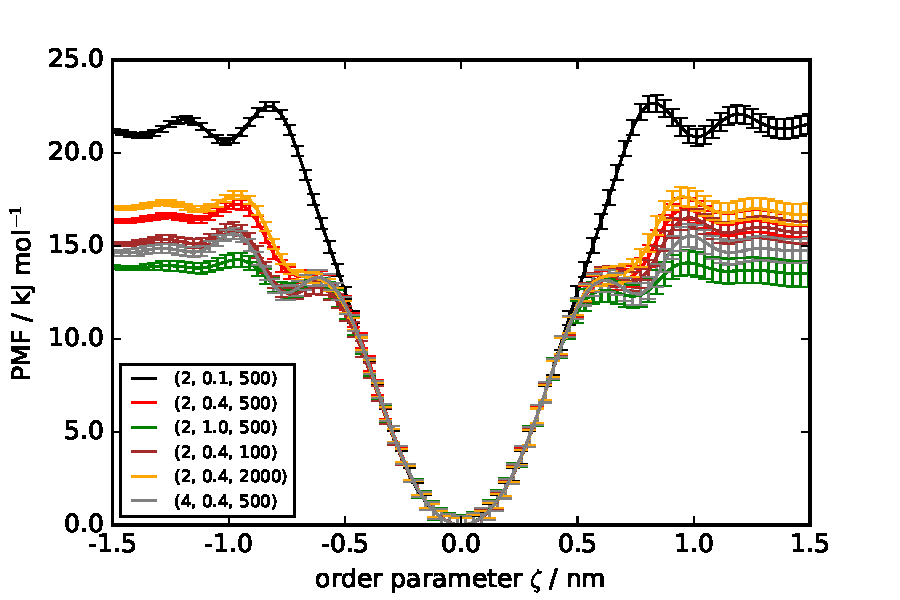
\includegraphics[width=\linewidth]{figures/pmf_uCNT_uMeth_transres.pdf}
\caption{
Effect of the orthogonal translational restraint on the PMF for methane / unpolar CNT.
Restraining parameters $(n, \rho_\mathrm{up} \, [\mathrm{nm}], k_\rho \, [\mathrm{kJ~mol}^{-1}~\mathrm{nm}^{-n}])$ as used for the flat-bottom potential $U_\rho$  according to Eq.~(\ref{eq:ort_restr}), 
are given by number triplets in the legend.
}
\label{fig:study_restr_host}
\end{figure}

\begin{table*}[ht]
\caption{\label{tbl:1Dsetup}
Influence of the translational restraint settings on the calculated standard binding free enthalpy $\Delta G^\circ_\mathrm{bind}$ for united-atom methane / unpolar CNT (c.f. Sec~\ref{res:UnpMet_UnpCNT}).
Corresponding PMFs are depicted in Fig.~\ref{fig:study_restr_host}. 
First three columns specify the parameters used for the flat-bottom potential $U_\rho$ (c.f. Eq.~(\ref{eq:ort_restr})). 
Calculations of $l_\mathrm{b}$, $A_{\mathrm{u},\rho}$ and $\Delta G^\circ_\mathrm{bind}$ were performed according to Eq.~(\ref{eq:lb}), Eq.~(\ref{eq:Au_2}) and Eq.~(\ref{eq:DG0_2}), respectively. 
The contribution of the translational restraint in the bound state $\Delta G_\rho$ was calculated using the MBAR estimator from a sequence of simulations in the bound state with force constants $k_\rho$ varying from zero to the final value as given above. Error estimates refer to the UI result.
}
\centering
\begin{tabular}{ccc ccc ccc}\hline
\multicolumn{3}{c}{Setup} &  \\
\cline{1-3} 
$n$ & $\rho_\mathrm{up}$ & $k_\rho$  & $\Delta W_\mathrm{R}$  & $l_\mathrm{b}$ & $A_{\mathrm{u},\rho}$ & $\Delta G_\mathrm{V}$ & 
$\Delta G_\rho$ & $\Delta G^\circ_\mathrm{bind}$ \\
$[-]$ & $[\mathrm{nm}]$ & $[\mathrm{kJ~mol}^{-1}~\mathrm{nm}^{-n}]$ & $[\mathrm{kJ~mol}^{-1}]$ & $[\mathrm{nm}]$ & $[\mathrm{nm}^2]$ & $[\mathrm{kJ~mol}^{-1}]$ & $[\mathrm{kJ~mol}^{-1}]$ & 
$[\mathrm{kJ~mol}^{-1}]$ \\ 
\hline
2 & 0.1 & 500  &  -21.37 $\pm$ 0.54 & 0.3827 &  0.1184 &  8.98  & -0.06 &  -12.44 $\pm$  0.54 \\   
2 & 0.4 & 500  &  -16.27 $\pm$ 0.62 & 0.3832 &  0.7565 &  4.35  & -0.13 &  -12.05 $\pm$  0.62\\
2 & 1.0 & 500  &  -13.80 $\pm$ 0.72 & 0.3869 &  3.7291 &  0.35  &  -0.14  &  -13.59 $\pm$ 0.72\\
2 & 0.4 & 100  &  -15.51 $\pm$ 0.61 & 0.3874 &  1.1569 &  3.27  &  -0.50 &  -12.74 $\pm$ 0.61\\
2 & 0.4 & 2000 & -16.93 $\pm$ 0.60 & 0.3835 &  0.6217 &  4.84  &  -1.03  &  -13.12 $\pm$ 0.60\\
4 & 0.4 & 500  &  -14.84 $\pm$ 0.66 & 0.3856 &  1.3047 &  2.98  &  -0.64 &  -12.50 $\pm$ 0.66\\ 
\hline
\end{tabular}
\end{table*}


\subsubsection*{Treatment of Electrostatic Interactions}

Fig.~\ref{fig:UU_Meth_CNT_electrst} shows the influence of different treatments for long-range electrostatics (PME vs. RF) alongside with different cut-off schemes (SR vs. TR) and pairlist generation schemes 
(CG vs. AT) on the PMF. As can be seen, all setups yield very similar PMFs. 
In Ref.~\citenum{baumketner2009removing}, a system size dependence of the PMF for ion association was observed in case of simulations based on the RF treatment. 
Therefore, additional simulations using box sizes of different x- and y-dimensions were conducted for the two TR-setups as well for the PME treatment (c.f. Tab.~\ref{tbl:overview_RF}). 
In all cases, no system size dependence could be observed  (data not shown).

\begin{figure}[htb!]
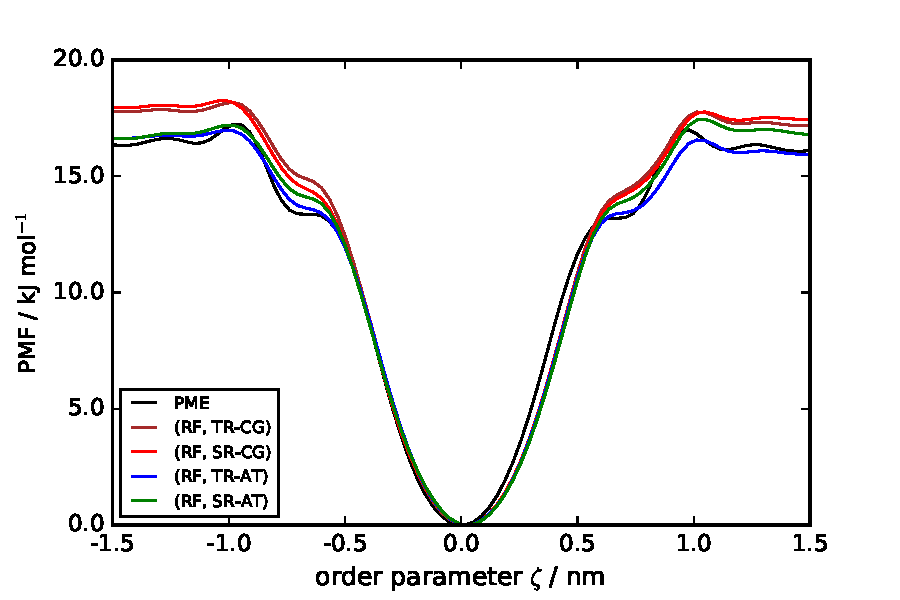
\includegraphics[width=\linewidth]{figures/pmf_uCNT_uMeth_electrostatics.pdf}
\caption{Effect of the treatment of electrostatic interactions (PME vs. RF), the cut-off scheme (SR vs. TR) and the pairlist generation scheme (CG vs. AT)  on the PMF for unpolar methane / unpolar CNT 
(c.f. Sec.~\ref{sec:simparam}).
Bounds for statistical uncertainties are below $1.0~\mathrm{kJ}~\mathrm{mol}^{-1}$ and have been omitted in the interest of clarity.
}
\label{fig:UU_Meth_CNT_electrst}
\end{figure}

\subsubsection*{Lesson Learned}

For the CNT / methane system, consistent PMFs were obtained leading to binding free enthalpies within maximal statistical bounds of 
$\pm 1.5~\mathrm{kJ}~\mathrm{mol}^{-1}$, regardless of how the host and the ligand's lateral movement was restrained (c.f. Tab.~\ref{tbl:1Dsetup}).
This conservative estimate for the maximal error encompasses the PMF uncertainty as delivered by the UI estimator as well as the spread of $\Delta G^\circ_\mathrm{bind}$ values obtained from the different setups. 
This distribution of $\Delta G^\circ_\mathrm{bind}$ values also emphasizes however, that even for such a simple system, no perfect agreement can be expected.
The treatment of electrostatic interactions and the pairlist generation scheme have an effect on $\Delta W_\mathrm{R}$ on the order of $\pm 1.5~\mathrm{kJ}~\mathrm{mol}^{-1}$.
These results are an important basis to judge the artifact reported in Sec.~\ref{subsec:pol_host_unp_lig}. 

%%%%%%%%%%%%%%%%%%%%%%%%%%%%%%%%%%%%%%%%%%%%%%%%%%%%%%%%%%%%

\subsection{Unpolar CNT / Multiatomic Ligand}
\label{subsec:unp_host_unp_lig}

This section reports the PMFs for the unpolar CNT host complexed with different multiatomic unpolar ligands.
Here, rigid diatomic ligands in the form of ethane and a modified model with increased bond length were studied as well as hexane.
In contrast to (ordinary) ethane, the elongated variant (in the remainder denoted as "elongated ethane")  is incapable to rotate inside the CNT cavity once it is bound.
This ligand selection enables to study the impact of the ligand's flexibility and rotational degrees of freedom inside the binding pose. 
Since it was found that all three estimators (WHAM, UI, MBAR) yield indistinguishable PMFs within errors bars, only the UI results will be reported in the following.


\subsubsection*{Restraining the Ligand's Orientation}
\label{subsubsec:orirest}

In practice it can often be essential to restrain not only the translational movement of the ligand but also its orientation towards the host molecule (c.f. Sec.~\ref{subsec:pol_host_pol_lig}).
Fig.~\ref{fig:OriRest} shows the PMFs for (a) ethane, elongated ethane and (b) hexane, obtained from the setup with (red curves) and without (black curves) orientational restraint.
As can be seen, the restraint on the ligand's rotation leads to higher absolute numbers of $\Delta W_\mathrm{R}$.
Comparison of the diatomic ligands shows that this increase is more pronounced for increasing bond lengths.
Tab.~\ref{tbl:unpLigOR} contains the calculated estimates for $\Delta G^\circ_\mathrm{bind}$. 
For each ligand, two estimates are provided, corresponding to the setup with and without orientational restraint. 
As revealed by the data, the application of an orientational restraint in case of ethane has a marginal effect on $\Delta W_\mathrm{R}$ but the free energy contribution from releasing this restraint in the bound state is the highest for all ligands.
The fact this contribution is almost identical for the bound and unbound state shows that the confinement inside the host's cavity has no significant effect on the populated ligand orientations in this case, as expected.
For elongated ethane and hexane, which are not able to rotate in the bound state, the free energy gain of releasing the restraint is much smaller.
The good agreement of the corresponding values for $\Delta G^\circ_\mathrm{bind}$ from simulations with and without orientational restraint confirms consistency between the setups. 
Results from double decoupling which was performed for ethane and elongated ethane, was also found to be in good accordance with the PMF-based estimates (c.f. Tab.~\ref{tbl:DDM}).
We conclude that the effect of an orientational restraint included in the simulation protocol with respect to the calculation of $\Delta G^\circ_\mathrm{bind}$ is captured adequately by the terms $\Delta G_\Omega$ and 
$\Delta G_\theta$ in Eq.~(\ref{eq:DG0_2}).
Therefore, a variation of the restraining force constant $k_\theta$ was not performed in this work.

\begin{figure}[htb!]
  \centering    
  \subfigure[]{\label{fig:a}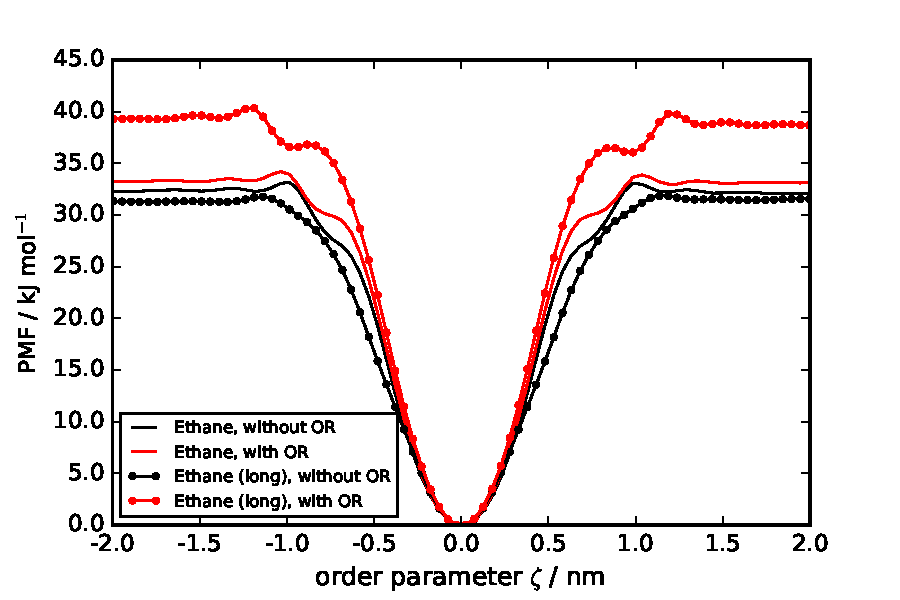
\includegraphics[width=\linewidth]{figures/pmf_uCNT_uEth_orires.pdf}}
  \subfigure[]{\label{fig:b}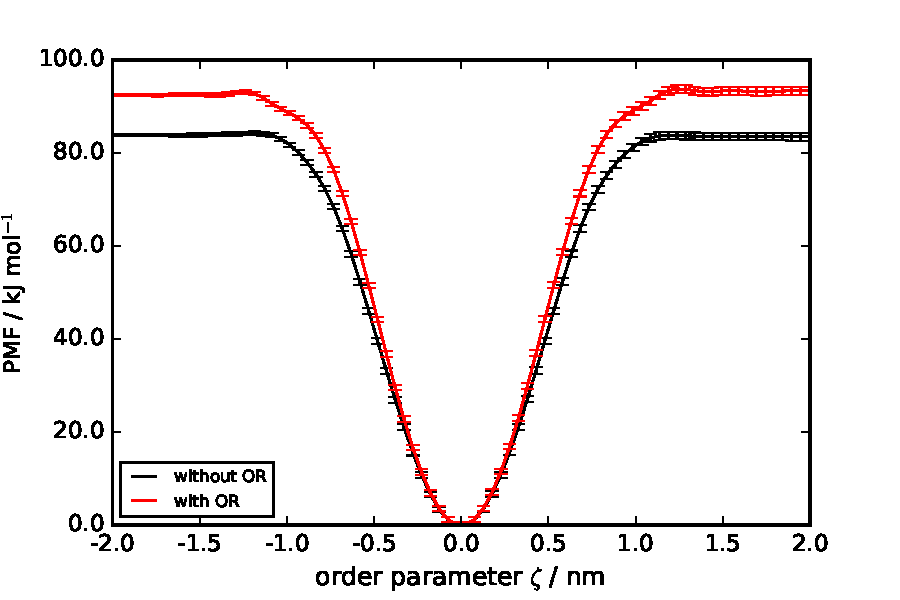
\includegraphics[width=\linewidth]{figures/pmf_uCNT_uHex_orires.pdf}}
  \caption{Effect of a restrained ligand orientation on the PMFs for (a) unpolar (elongated) ethane / unpolar CNT 
  and (b) unpolar hexane / unpolar CNT.
  Red and black curves correspond to PMFs obtained from the setup with and without orientational restraint (OR), respectively.
  Error bars in graph (a) have been omitted in the interest of clarity.
  }
  \label{fig:OriRest}
\end{figure}

\begin{table*}[ht]
\caption{\label{tbl:unpLigOR} 
Calculated standard binding free enthalpies $\Delta G^\circ_\mathrm{bind}$ for the binding of unpolar ethane, elongated ethane and hexane to the unpolar CNT (c.f. Sec~\ref{subsec:unp_host_unp_lig}).
Two rows of data are associated with every ligand, corresponding to the setup with and without orientational restraint (OR).
Corresponding PMFs are depicted in Fig.~\ref{fig:OriRest}. 
Calculations of $l_\mathrm{b}$,  $\Delta G_\mathrm{V}$ and $\Delta G_\Omega$ were performed as described in Sec.~\ref{sec:theory_DG0}. 
The joint contribution of the translational and orientational restraint in the bound state ($\Delta G_\rho + \Delta G_\theta$) was calculated using the MBAR estimator from a sequence of simulations in the bound state with force constants $k_\rho$ and $k_\theta$ varying from zero to the final values as specified in Tab.~\ref{tbl:restr_1}. 
The estimate of $\Delta G^\circ_\mathrm{bind, Conf. 1}$ as obtained from the setup including an orientational restraint corresponds to one distinct binding configuration and was corrected 
by a symmetry term of $-RT \ln 2$~\cite{gilson2013correction, hermans1997inclusion} to obtain $\Delta G^\circ_\mathrm{bind}$ in case of elongated ethane and hexane 
due to their incapability to rotate inside the CNT cavity in the absence of orientational restraint (c.f. Sec.~\ref{sec:application}). 
Error estimates refer to the UI result.
}
\centering
\begin{tabular}{llc ccc ccc}\hline
System & Setup & $\Delta W_\mathrm{R}$  & $l_\mathrm{b}$ & $\Delta G_\mathrm{V}$ & $\Delta G_\Omega$ & 
$\Delta G_\rho + \Delta G_\theta$ & $\Delta G^\circ_\mathrm{bind, Conf. 1}$ & $\Delta G^\circ_\mathrm{bind}$ \\
& & $[\mathrm{kJ~mol}^{-1}]$ & $[\mathrm{nm}]$ &  $[\mathrm{kJ~mol}^{-1}]$ & $[\mathrm{kJ~mol}^{-1}]$ & $[\mathrm{kJ~mol}^{-1}]$ & $[\mathrm{kJ~mol}^{-1}]$ & $[\mathrm{kJ~mol}^{-1}]$ \\ 
\hline
\multirow{ 2}{*}{Ethane}  		& No OR 	& -32.16 $\pm$ 0.87 	& 0.2989 	&  4.97 	&  0.00 	&  0.00 	&  -  					& -27.19 $\pm$ 0.87 \\   
						& OR       	& -33.23 $\pm$ 0.74 	& 0.2925  	&  5.03 	&  14.95	&  -14.41 	&  -27.66 $\pm$ 0.74  	& -27.66 $\pm$ 0.74 \\ 
\hline
\multirow{ 2}{*}{Long Ethane}  	& No OR 	& -31.38 $\pm$ 0.85 	& 0.2864 	&  5.08 	&  0.00 	&  0.00 	&  -  					& -26.30 $\pm$ 0.85 \\    
					      	& OR       	& -38.97 $\pm$ 0.81 	& 0.2707  	&  5.22 	&  14.95 	&  -5.65 	&  -24.44 $\pm$ 0.81  	& -26.17 $\pm$ 0.81\\ 
\hline
\multirow{ 2}{*}{Hexane}  		& No OR 	& -83.65 $\pm$ 0.89 & 0.1995 	&  5.98 	&  0.00 	&  0.00 	&  -  					& -77.67 $\pm$ 0.89\\  
						& OR       	& -92.99 $\pm$ 0.92 & 0.1954  &  6.03 	&  14.95 	&  -4.72 	&  -76.72 $\pm$ 0.92  	& -78.45 $\pm$ 0.92\\   
\hline
\end{tabular}
\end{table*}


\subsubsection*{Choice of Restraining Reference Points}
\label{subsec:refpoints}

The decision which (pseudo) atoms to choose in the host and ligand molecule to serve as reference or anchor points for the applied distance restraint in the Umbrella Sampling simulations is often not clear a priori.
Though the centers of mass might be an intuitive choice (and were selected for the majority of studies of the current work), other choices might appear more suitable in practical application~\cite{doudou2009standard}.
Fig.~\ref{fig:refpoints} (a) and (b) show the PMFs for elongated ethane / CNT and hexane / CNT, respectively, as obtained when a peripheric carbon atom was picked as reference point in the ligand.
The COM of the CNT was chosen as reference point within the host as has been the case hitherto.  
Every graph contains two free energy profiles, corresponding to the PMF evaluated with (red curves) and without (black curves) orientational restraint.
In the setup lacking an orientational restraint, a substantial free energy offset between 20 (elongated ethane) and 55~kJ~mol$^{-1}$ (hexane) is present in the PMF.
The reason for this offset lies in the differences of the sampled configurational space at the two pore mouths. 
Depending on which part of the ligand is buried (the part with or without the anchor atom for the distance restraint), the configurational space accessible to the partly bound ligand is quite different. 
The estimation of  $\Delta G^\circ_\mathrm{bind}$ from such a PMF would lead to very different results depending on which branch of the PMF would have been taken as a basis for the analysis.
In contrast, if the COM of the ligand is chosen as anchor atom, the rotational behavior of the ligand is symmetric at both CNT ends and no PMF offset is present, even when the ligand's orientation is not restrained 
(c.f. Fig.~\ref{fig:OriRest}). 
However, as demonstrated in Fig.~\ref{fig:refpoints}, even in case of such an "unfortunate" choice of anchor points, the PMF offset can be eliminated through the usage of an orientational restraint.
Comparison of the corresponding profiles of Fig.~\ref{fig:refpoints} and Fig.~\ref{fig:OriRest} obtained from the setup including an orientational restraint (but different reference points in the ligand), 
shows that the PMFs are identical except for a marginal shift along the order parameter axis which will not affect the estimate for $\Delta G^\circ_\mathrm{bind}$.

\begin{figure}[htb!]
  \centering    
  \subfigure[]{\label{fig:a}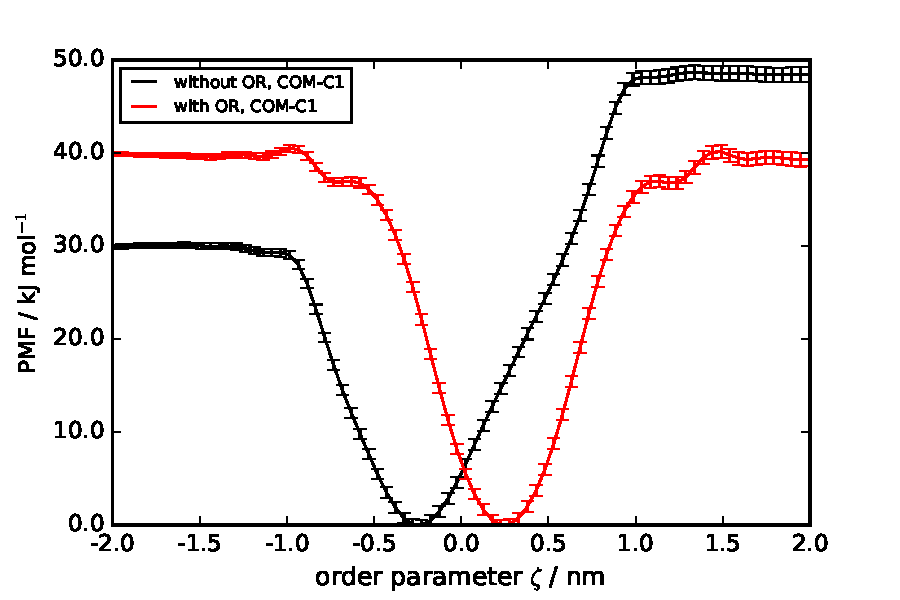
\includegraphics[width=\linewidth]{figures/pmf_uCNT_uEth_refpoint.pdf}}
  \subfigure[]{\label{fig:b}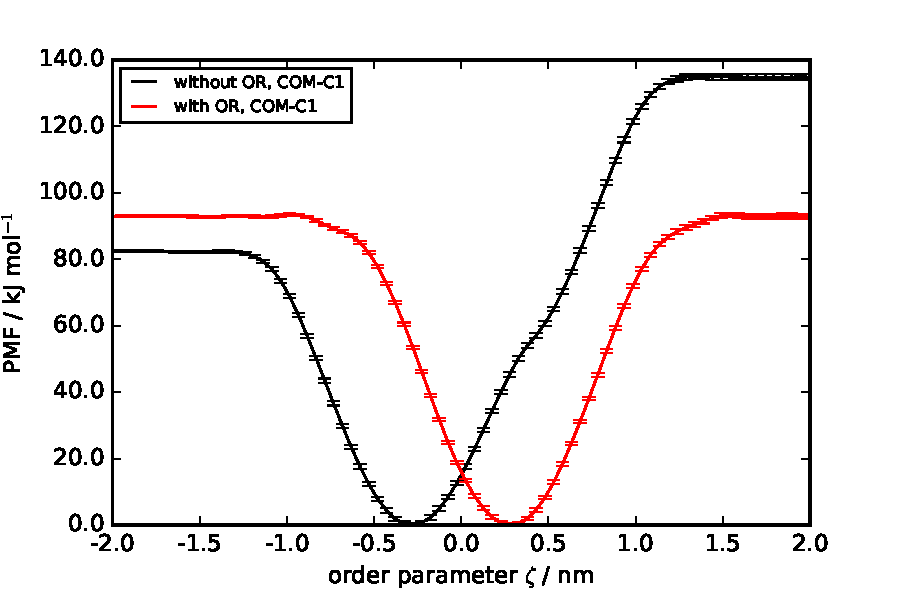
\includegraphics[width=\linewidth]{figures/pmf_uCNT_uHex_refpoint.pdf}}
  \caption{
  Effect of the choice of reference points for the distance restraint on the PMFs for (a) unpolar elongated ethane / unpolar CNT and (b) unpolar hexane / unpolar CNT.
  Here, the COM of the CNT and the C1 carbon atom of the ligand was chosen as reference points.
  Red and black curves correspond to PMFs obtained from the setup with and without orientational restraint (OR), respectively.
  }
  \label{fig:refpoints}
\end{figure}

\subsubsection*{Treatment of Electrostatic Interactions}

Fig.~\ref{fig:UU_MultiLig_CNT_electrst} shows the influence of the treatment for long-range electrostatics (PME vs. RF) alongside with the pairlist generation scheme (CG vs. AT) on the PMFs for two systems: 
(a) ethane / CNT and (b) hexane / CNT. 
In addition, the effect of different cut-off schemes (SR vs. TR) was tested in case of ethane / CNT.
In none of the cases, an orientational restraint was included in the protocol. 
As can be seen, all setups yield almost indistinguishable PMFs for ethane / CNT, whereas for hexane / CNT, the two RF setups yield a slightly narrower PMF well compared to the PME result. 
Referring to the effect on the binding free enthalpy, such a different shape only affects the calculation of the bound length $l_\mathrm{b}$ (c.f. Eq.~(\ref{eq:lb})) leading to a marginal 
discrepancy in the order of $\pm 0.5~\mathrm{kJ}~\mathrm{mol}^{-1}$ compared to the PME-based estimate.
As in case of methane / CNT, no system size dependence for the PMFs could be observed (data not shown).

\begin{figure}[htb!]
  \centering    
  \subfigure[]{\label{fig:a}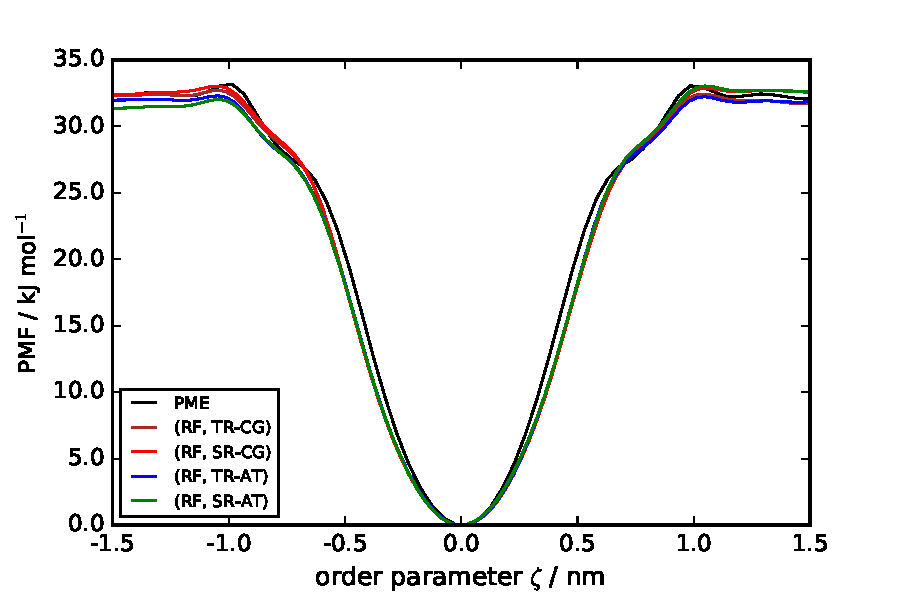
\includegraphics[width=\linewidth]{figures/pmf_uCNT_uEth_electrostatics.pdf}}
  \subfigure[]{\label{fig:b}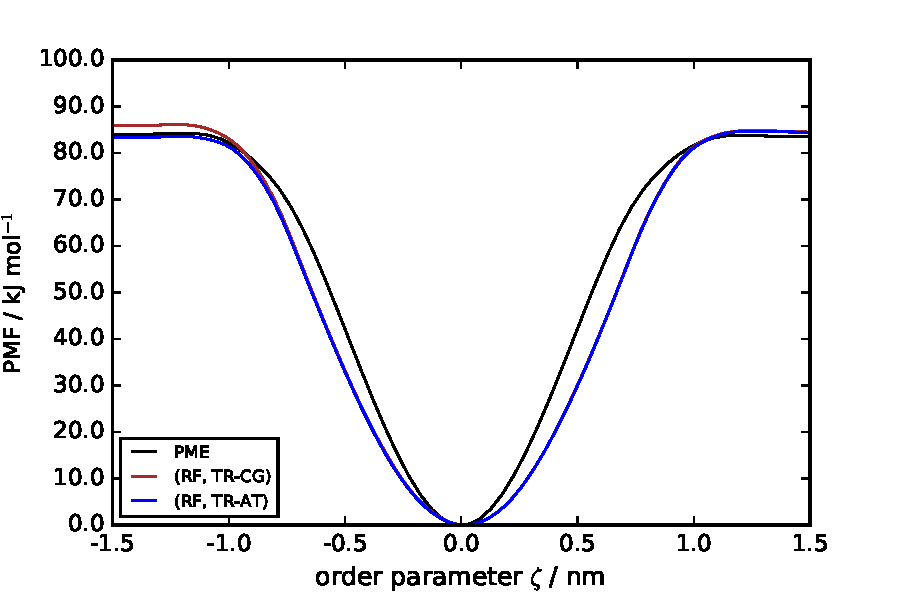
\includegraphics[width=\linewidth]{figures/pmf_uCNT_uHex_electrostatics.pdf}}
  \caption{Effect of the treatment of electrostatic interactions (PME vs. RF), the cut-off scheme (SR vs. TR) and the pairlist generation scheme (CG vs. AT) on the PMF for (a) unpolar ethane / unpolar CNT 
  and (b) unpolar hexane / unpolar CNT (c.f. Sec.~\ref{sec:simparam}). 
  No orientational restraint was applied to the ligands. 
  Bounds for statistical uncertainties are below $1.0~\mathrm{kJ}~\mathrm{mol}^{-1}$ and have been omitted in the interest of clarity.
}  
\label{fig:UU_MultiLig_CNT_electrst}
\end{figure}


\subsubsection*{Lesson Learned}

For the binding of symmetric unpolar multiatomic ligands to the unpolar CNT, the change in rotational entropy upon binding is included in the PMF if no orientational restraint is used.
The two setups (with and without orientational restraint) lead to standard binding free enthalpies which are indistinguishable within statistical uncertainties.
An orientational restraint is required however, if the anchor points for the Umbrella distance restraint in the ligand and in the CNT are chosen in such a way, 
that the configurational space accessible to the partly bound ligand at the both cavity entrances are different. 
The treatment of electrostatic interactions and the pairlist generation scheme have a marginal effect on $\Delta W_\mathrm{R}$ on the order of $\pm 1~\mathrm{kJ}~\mathrm{mol}^{-1}$.

%%%%%%%%%%%%%%%%%%%%%%%%%%%%%%%%%%%%%%%%%%%%%%%%%%%%%%%%%%%%
\subsection{Polar CNT / Unpolar Ligand}
\label{subsec:pol_host_unp_lig}

This section reports PMFs for the association of a polar CNT with different unpolar ligands.
The polar CNT was modeled by distributing balancing charges to terminal pairs of C-H-atoms at one side of the CNT (C-atoms: -0.5~e, H-atoms: +0.5~e where "e" denotes the elementary charge).
Every balancing pair of C-H atoms was assigned to one neutral charge group in case of simulations based on the RF approach for long-range electrostatics in combination with the CG pairlist scheme.
In contrast to the unpolar systems treated so far, care has to be taken in order to avoid a bias due to the applied PMF analysis method. 
This issue is discussed explicitly in a separate subsection. 

\subsubsection*{Impact of the Host's Polarity}

Fig.~\ref{fig:polCNT_unpLig} shows PMFs for a set of unpolar ligands (methane, (elongated) ethane, hexane) binding to the polar CNT. 
No orientational restraint was imposed on the ligand.
In contrast to the previous examples corresponding to the binding to an unpolar CNT, the resulting PMFs are highly asymmetric featuring a considerable barrier to be overcome by the ligand at the polar entrance of the CNT. 
This barrier which is caused by the modified water structure in proximity to the polar mouth, makes the binding path through that particular side energetically unfavorable.
\begin{figure}
  \centering    
  \subfigure{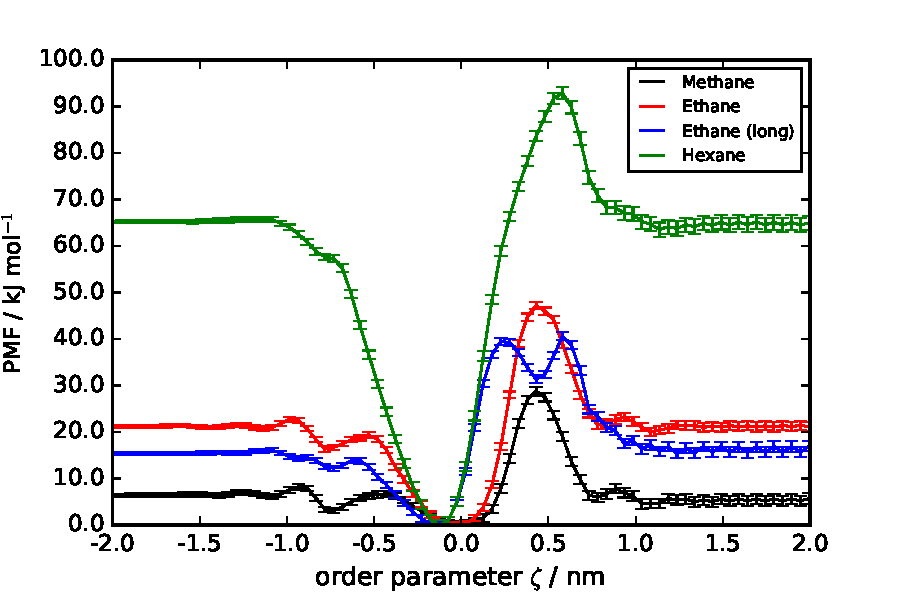
\includegraphics[width=\linewidth]{figures/pmf_pCNT_uLig_NoOR.pdf}}
  \caption{
  PMFs for the association of a polar CNT with different unpolar ligands. No orientational restraint was imposed on the ligand. 
  Long-range electrostatic interactions were treated with the PME method. PMFs were estimated via the UI method.
  }
  \label{fig:polCNT_unpLig}
\end{figure}

\subsubsection*{Treatment of Electrostatic Interactions}

Fig.~\ref{fig:UP_LigCNT_electrst} shows the influence of the treatment for long-range electrostatics (PME vs. RF) 
alongside with the pairlist generation scheme (CG vs. AT) and cut-off scheme (SR vs. TR) on the PMFs for two systems: (a) methane / polar CNT and (b) unpolar ethane / polar CNT. 
In case of ethane, no orientational restraint was applied. 
As can be seen, PMFs based on an atomistic interaction scheme (TR-AT, SR-AT) show a smaller well (measured by $\Delta W_\mathrm{R}$) and barrier at the polar entrance 
compared to analogue simulations based on charge groups (TR-CG, SR-CG).
The combination of the RF approach with an atomistic interaction scheme also shows higher resemblance with the PME solution as judged by the value of $\Delta W_\mathrm{R}$.
We found that typically much longer simulations times (more than 40~ns per window) were required compared to PME-based simulations (typically 20~ns per window were sufficient) in order to achieve converged estimates. 
No significant impact of the underlying cut-off schemes (SR vs. TR) could be observed.
As in the previous sections, no systematic system size dependence was found.

\begin{figure}[htb!]
  \centering    
  \subfigure[]{\label{fig:a}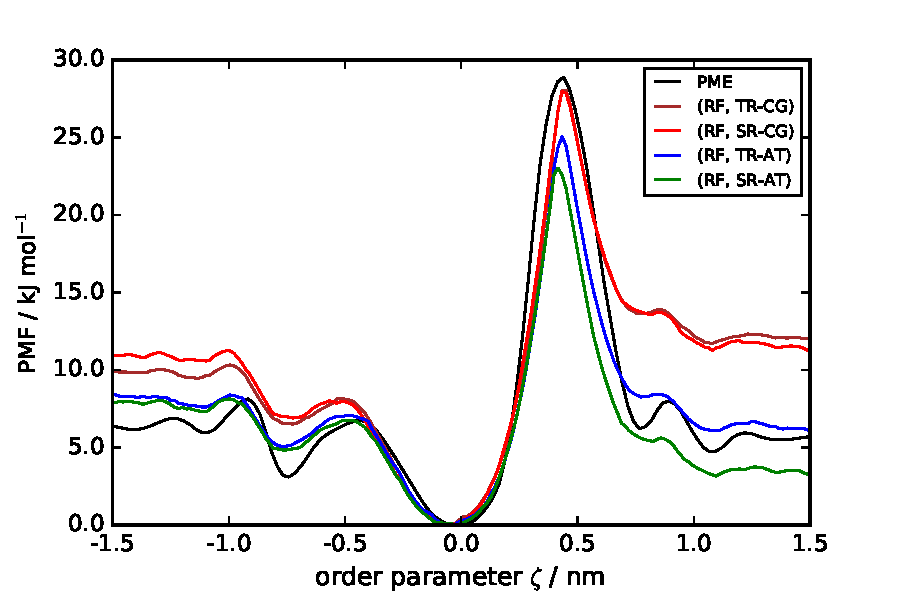
\includegraphics[width=\linewidth]{figures/pmf_pCNT_uMeth_electrostatics_WHAM.pdf}}
  \subfigure[]{\label{fig:b}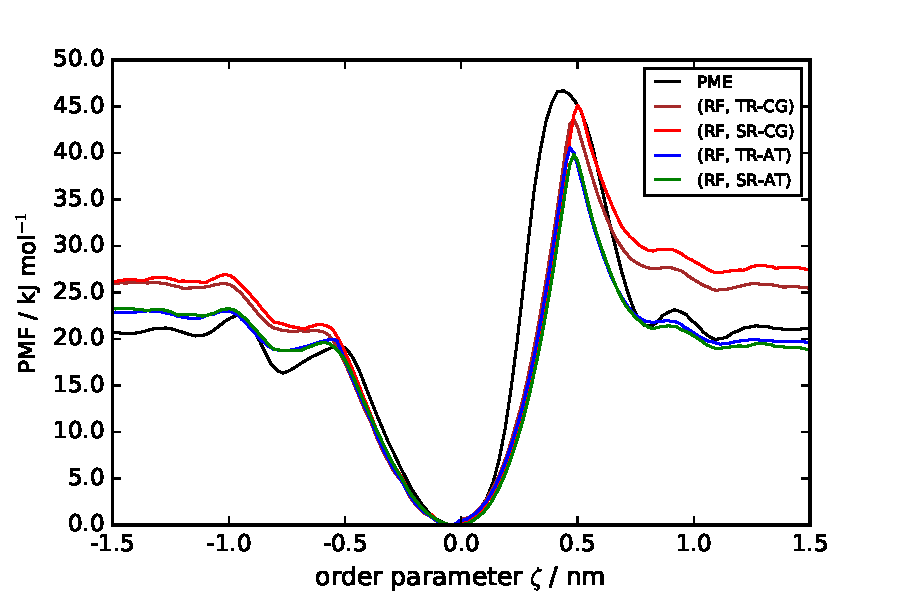
\includegraphics[width=\linewidth]{figures/pmf_pCNT_uEth_electrostatics_WHAM.pdf}}
  \caption{Effect of the treatment of electrostatic interactions (PME vs. RF), the cut-off scheme (SR vs. TR) and the pairlist generation scheme (CG vs. AT) on the PMF for (a) methane / polar CNT 
  and (b) unpolar ethane / polar CNT (c.f. Sec.~\ref{sec:simparam}). 
  No orientational restraint was applied for ethane. 
  PMFs were estimated via the WHAM method.
  Error bars have been omitted in the interest of clarity. 
}  
\label{fig:UP_LigCNT_electrst}
\end{figure}


\subsubsection*{Impact of the Free Energy Estimator}

For the considered systems unpolar ligand / polar CNT it was found that artifacts in the form of a PMF offset as detected previously in another context (c.f. Sec.~\ref{subsec:refpoints}), can be introduced by the analysis method. 
Fig.~\ref{fig:polCNT_unpLig_estimator} shows a comparison between PMFs as obtained from different estimators (UI, WHAM, MBAR) for the example of unpolar ethane / polar CNT based on the (RF, TR-CG) setup.
As can be seen, an offset between the flat bulk water regions of around 7~kJ~mol$^{-1}$ is present in the profile obtained from the UI method, which significantly exceeds bounds due to the statistical uncertainty.
Its origin can be explained by means of the sampled biased distribution functions of the order parameter $\zeta$ 
(c.f. Fig.~\ref{fig:polCNT_unpLig_estimator_distrib}). 
As noted previously in Sec.~\ref{sec:estimators}, a central assumption in the UI approach is that the biased distributions can be approximated as Gaussian distributions.
In Fig.~\ref{fig:polCNT_unpLig_estimator_distrib} (a) it can be seen that the distribution sampled from window close to $\zeta =0.5~\mathrm{nm}$ at the polar CNT entrance differs from the rest and is non-Gaussian in shape.
The set of distributions from corresponding PME-based simulation in contrast, does not contain such a window (c.f. Fig.~\ref{fig:polCNT_unpLig_estimator_distrib} (b)).
Such an offset was exclusively observed for simulations based on the reaction field treatment (including different ligands and combinations of cut-off and pairlist generation schemes) 
which is more susceptible for cut-off artifacts in structural solvation properties~\cite{reif2011computation} 
but not for PME-based simulations.
Nonetheless, we stress that this artifact is only indirectly caused by the electrostatics treatment but actually results from application of an estimator to a situation for which it was not designed for.
The usage of a higher force constant for the Umbrella distance restraint might probably remedy such a bias.


\begin{figure}
  \centering    
  \subfigure{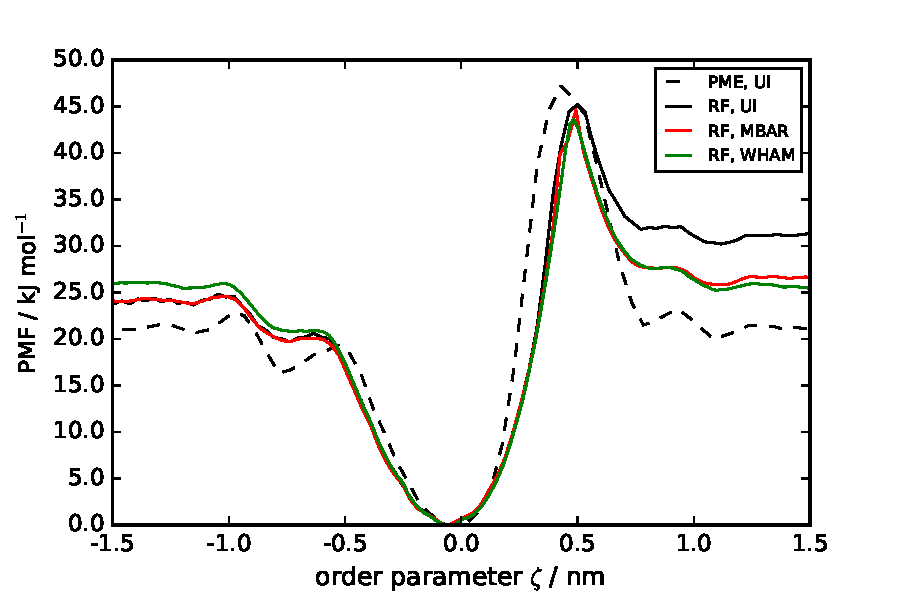
\includegraphics[width=\linewidth]{figures/pmf_pCNT_uEth_CGTR_box2_estimators.pdf}}
  \caption{
  Influence of the free energy estimator (UI vs. MBAR vs. WHAM) on the PMF for unpolar ethane / polar CNT. 
  Electrostatics treatment refers to the (RF, TR-CG) setup as described in the main text. The profile obtained from simulations using PME and evaluated via UI is shown for comparison (black dashed line).
  No orientational restraint was imposed on the ligand. 
  }
  \label{fig:polCNT_unpLig_estimator}
\end{figure}

\begin{figure}[htb!]
  \centering    
  \subfigure[]{\label{fig:a}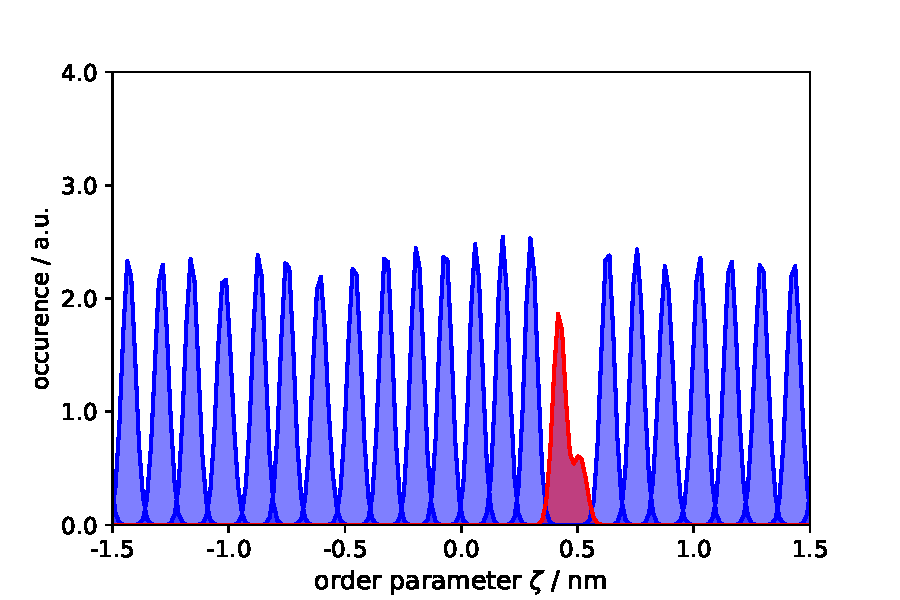
\includegraphics[width=\linewidth]{figures/histo_pCNT_uEth_CGTR_box2.pdf}}
  \subfigure[]{\label{fig:b}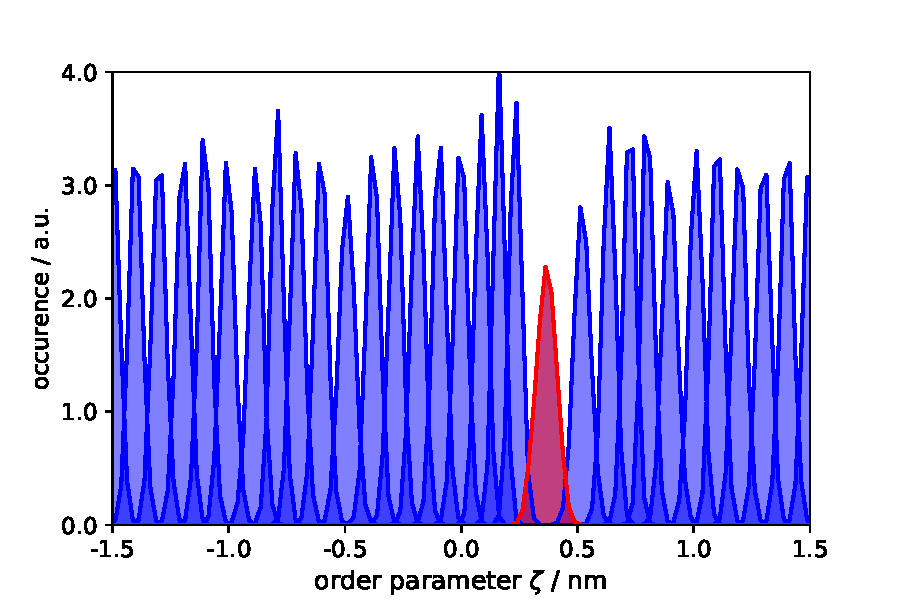
\includegraphics[width=\linewidth]{figures/histo_pCNT_uEth_PME.pdf}}
  \caption{
  Influence of electrostatics treatment on sampled biased distributions of the order parameter $\zeta$ along the considered path for unpolar ethane / polar CNT. 
  (a): RF-based simulations using the TR-CG setup, (b): PME-based simulations. The distribution close to $\zeta =0.5~\mathrm{nm}$ is highlighted in red to support the discussion in the main text. 
  The abbreviation a.u. refers to arbitrary units.
}  
\label{fig:polCNT_unpLig_estimator_distrib}
\end{figure}


\subsubsection*{Lesson Learned}

The examples show that also in the presence of considerable polar interactions between host and solvent, 
neither the differences in the treatment of electrostatic interactions nor in schemes for the cut-off or pairlist generation affect the estimated PMFs systematically.
The  artifact caused by the UI estimator demonstrates the benefit to compare different analysis methods on the same data set.
Furthermore, if the UI estimator is used, the shape of the sampled distributions should be checked.

%%%%%%%%%%%%%%%%%%%%%%%%%%%%%%%%%%%%%%%%%%%%%%%%%%%%%%%%%%%%
\subsection{Polar CNT / Dipolar Ligand}
\label{subsec:pol_host_pol_lig}

This section reports PMFs for the association of a polar CNT with different dipolar ligands based on (elongated) ethane and hexane.
The modeling of the polar CNT was described in the previous section. 
Dipolar ligands were modeled in a similar way by distributing a pair of balancing partial charges  to the peripheric pair of covalently bound carbon atoms 
(C1-atom: +0.5~e, C2-atom: -0.5~e where "e" denotes the elementary charge).
For all simulations considered in this paragraph, the PME treatment for long-range electrostatics was utilized.
Since it was found that the different estimators (WHAM, UI, MBAR) yield indistinguishable PMFs within errors bars, all profiles reported in the following refer to the UI result.

\subsubsection*{Sampling of Ligand Orientations}

In contrast to the systems treated so far, two distinct binding configurations with different binding affinities can be distinguished. 
The bound configuration for which the positively charged ligand head (C1-atom) is facing (away from) the negatively charged C-atoms of the CNT is denoted as Conf.~1 (Conf.~2).
PMFs for dipolar ethane, elongated ethane and hexane binding to the polar CNT are depicted in Fig.~\ref{fig:polCNT_polLig}.  
Profiles in (a) and (b) were obtained without and with imposed orientational restraint on the ligand, respectively.
For all simulations, the dipolar ligand was initially prepared in Conf.~1.
Significant differences become apparent from comparison with corresponding profiles in Fig.~\ref{fig:polCNT_unpLig} where the ligands "feel" the influence of the polar CNT only in an indirect manner mediated by the solvent.
Fig.~\ref{fig:polCNT_polLig} (a) reveals substantial PMF offsets of 10 and 60~kJ~mol$^{-1}$ for hexane and elongated ethane, respectively, both of which are incapable to rotate inside CNT.
For ethane in contrast, which can rotate inside the CNT due to its small size, no offset is present. 
As demonstrated by Fig.~\ref{fig:polCNT_polLig} (b), such an offset can be removed for all considered ligands through inclusion of an orientational restraint in the simulation protocol.

\begin{figure}[htb!]
  \centering    
  \subfigure[]{\label{fig:a}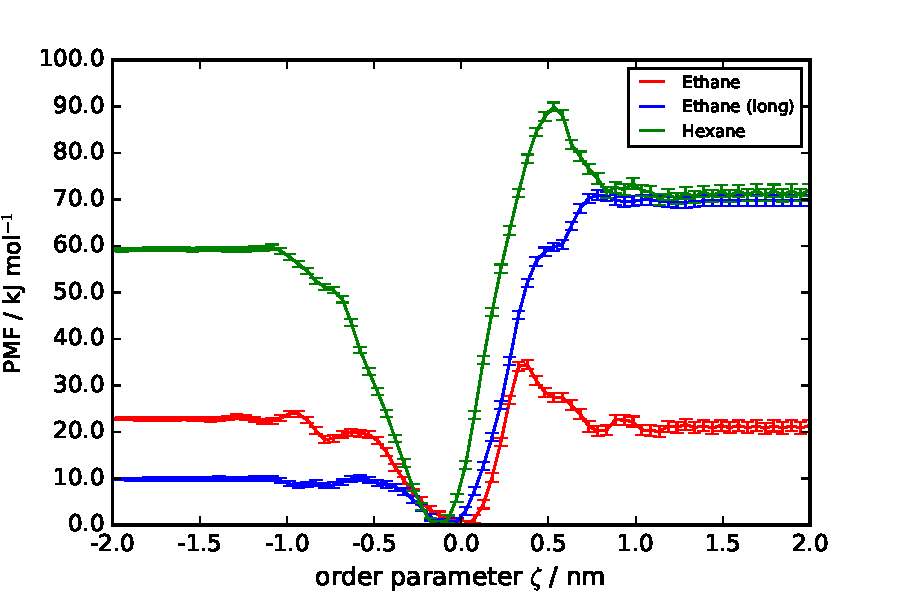
\includegraphics[width=\linewidth]{figures/pmf_pCNT_pLig_NoOR.pdf}}
  \subfigure[]{\label{fig:b}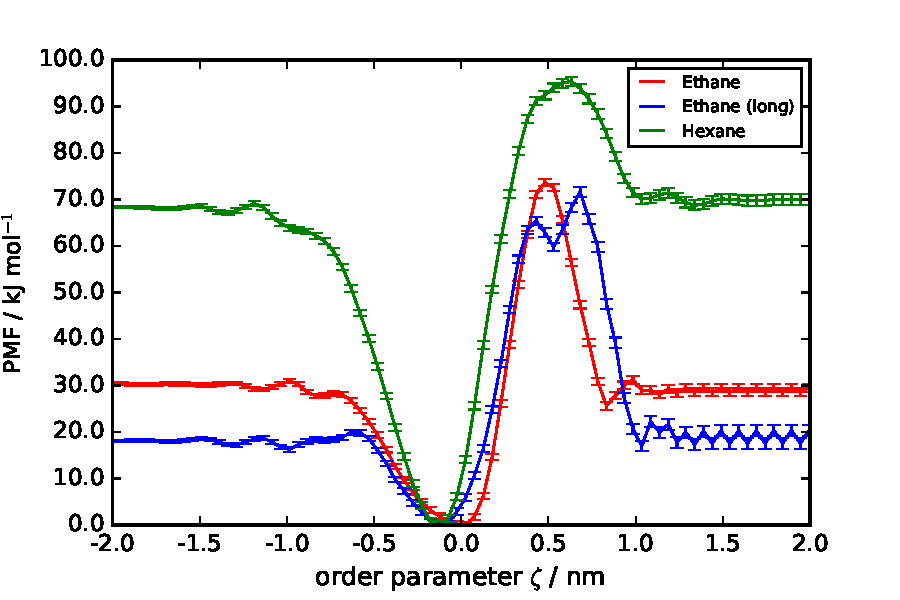
\includegraphics[width=\linewidth]{figures/pmf_pCNT_pLig_OR.pdf}}
  \caption{
  PMFs for the association of a polar CNT with different dipolar ligands. 
  All ligands were initially prepared in the same binding configuration (Conf.~1).
  Profiles in (a) and (b) refer to the setup without and with imposed orientational restraint on the ligand, respectively.
  }
  \label{fig:polCNT_polLig}
\end{figure}

\subsubsection*{Lesson Learned}

The examples illustrate that in case of asymmetric ligands binding to an asymmetric host (which is probably the most common case in practice), 
the biased distributions sampled in Umbrella windows outside the binding site in which the ligand is free to rotate does not fit to the biased distributions sampled in windows for the bound state 
in which the binding pose is prescribed. This misfit can be illustrated by excluding configurations exhibiting the "wrong" orientation from the analysis which reduces the offset considerably (data not shown). 
We point out that excluding states from the analysis was done just to support our findings, and is not meant to be a suitable method to avoid offsets. 
The use of an orientational restraint is therefore mandatory in such cases unless the Umbrella Sampling is combined with Hamiltonian Replica Exchange as discussed in the following section.

%%%%%%%%%%%%%%%%%%%%%%%%%%%%%%%%%%%%%%%%%%%%%%%%%%%%%%%%%%%%
\subsection{Cyclodextrin / Alcohols}
\label{sec:application}

This section reports PMFs for the association of $\alpha$-cyclodextrin ($\alpha$CD) with two different primary alcohols (1-butanol, 1-dodecanol).
Results for further alcohols were reported in our previous work~\cite{markthaler2017molecular}.
Since it was found that the different estimators (WHAM, UI, MBAR) yield indistinguishable PMFs within errors bars, all profiles reported in the following refer to the UI result.

\subsubsection*{Sampling of Ligand Orientations}

As in the case of dipolar ligands binding to the polar CNT, two different binding configurations can be distinguished which will be denoted as Conf.~1 and Conf.~2 according to Refs.~\citenum{markthaler2017molecular} and \citenum{gebhardt2016calculation}.
Fig.~\ref{fig:PMF_aCD} (a) and (b) show the PMFs for 1-butanol and 1-dodecanol binding to $\alpha$CD, respectively. 
Each graph contains two PMFs, corresponding to the setup with (red curve) and without (black curve) orientational restraint with the ligand bound to $\alpha$CD (Conf.~1).
The third profile (green curve) in both graphs corresponds to the PMFs as obtained from Umbrella Sampling combined with Replica Exchange (RE-US)~\cite{sugita2000multidimensional}. 
In RE-US, the Hamiltonians of neighboring windows defined by the individual values for the bias centers are allowed to swap after predefined time instances, based on the Metropolis-Hastings criterion. 
Here, an exchange was attempted every 1000 steps.  
For RE-US simulations, no orientational restraint was applied. 
A significant offset is visible for the PMFs lacking an orientational restraint. 
As observed previously in case of the dipolar ligand / polar CNT system (c.f. Sec.~\ref{subsec:pol_host_pol_lig}), this offset can be remediated by restricting the ligand orientation.
The fact that also the RE-US approach (without orientational restraint) yields an offset-free PMF, further demonstrates that this artifact is caused by a bias introduced when prescribing the binding pose in standard Umbrella Sampling.

The estimate of the binding free enthalpy as obtained from the protocol including an orientational restraint, corresponds to one particular binding configuration (in this case Conf.~1) and should be therefore denoted as 
$\Delta G^\circ_\mathrm{bind, Conf. 1}$.
For comparison with experiments which measure a configurational average, the binding free enthalpy for the second binding configuration 
(obtained from additional simulations and denoted as $\Delta G^\circ_\mathrm{bind, Conf. 2}$) can be combined with $\Delta G^\circ_\mathrm{bind, Conf. 1}$ via exponential averaging~\cite{mobley2006use}:
\begin{equation}
\Delta G^\circ_\mathrm{bind} = -RT \ln\left(   \mathrm{e}^{-\Delta G^\circ_\mathrm{bind, Conf. 1}/RT}  +  \mathrm{e}^{-\Delta G^\circ_\mathrm{bind, Conf. 2}/RT}  \right)
\label{eq:ExpAv_1}
\end{equation}
In RE-US simulations (without orientational restraint) in contrast, both binding configurations are sampled and the corresponding 
PMF can not be attributed to either Conf.~1 or Conf.~2 but already represents a configurational average.
Thus, the estimate for $\Delta G^\circ_\mathrm{bind}$ inferred from such a PMF can be directly compared with the corresponding experimental value without the need of  additional simulations. 
However, this gain in efficiency might be offset by an overhead in terms of hardware resources and (depending on the system) computation time for reaching convergence.  
Here, it was found that in case of butanol 20~ns per window were sufficient to obtain converged PMFs while 140~ns per window were required for dodecanol.
For standard Umbrella Sampling including an orientational restraint in contrast, 20~ns per window were found to be sufficient for all systems, at least in case of simulations based on the PME treatment for 
long-range electrostatics as mentioned previously.  
The good agreement between the $\Delta G^\circ_\mathrm{bind}$ estimates obtained from the setup including an orientational restraint and the RE-US simulations (c.f. Tab.~\ref{tbl:aCD})  
indicates that the RE scheme not only removes the PMF artifact but especially samples both binding configurations with the correct weighting.
Moreover, the results were found to be in good agreement with corresponding estimates from double decoupling (c.f. Fig.~5 in Ref.~\citenum{markthaler2017molecular}). 


\begin{figure}[htb!]
  \centering    
  \subfigure[]{\label{fig:a}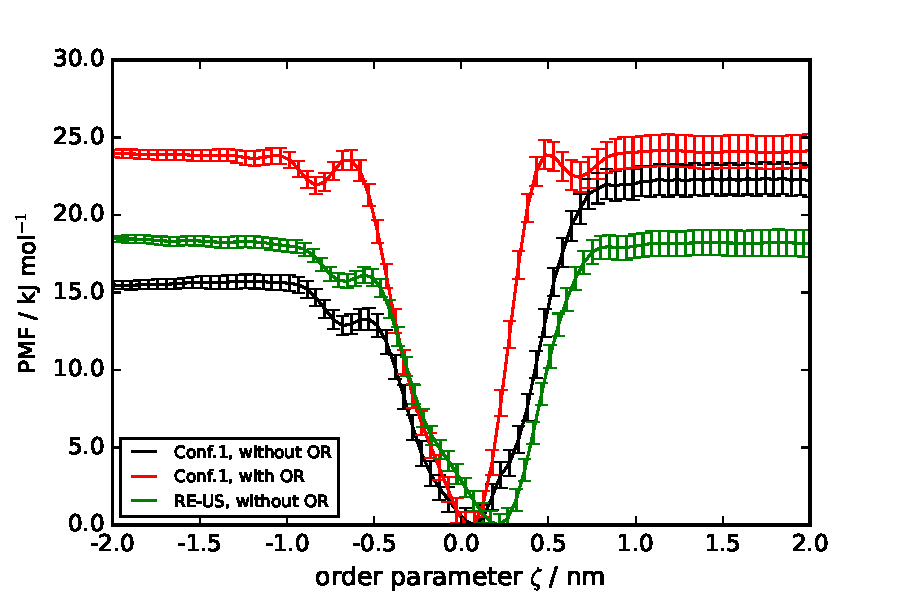
\includegraphics[width=\linewidth]{figures/pmf_aCD_BTL.pdf}}
  \subfigure[]{\label{fig:b}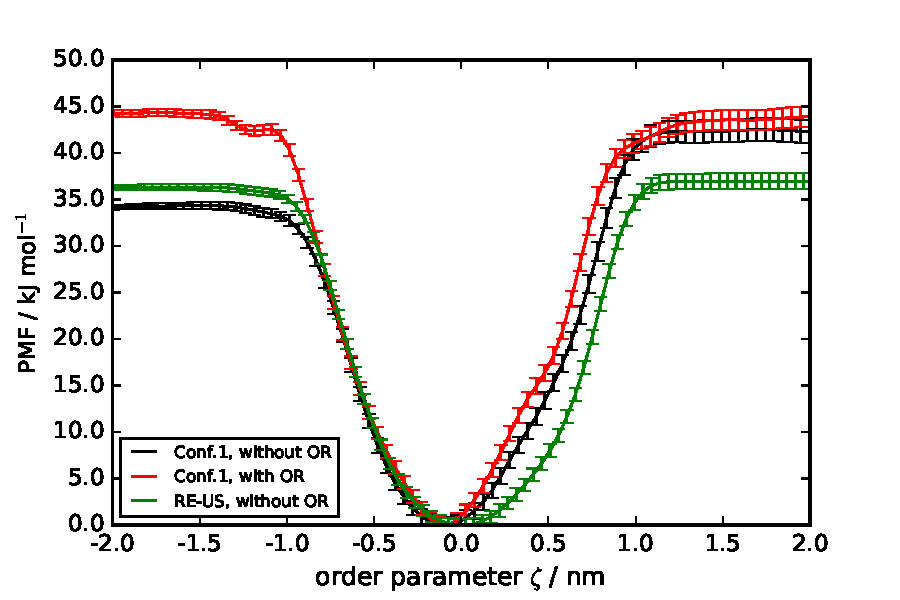
\includegraphics[width=\linewidth]{figures/pmf_aCD_DDL.pdf}}
  \caption{PMFs for (a) 1-butanol and (b) 1-dodecanol binding to $\alpha$CD (Conf.1)~\cite{markthaler2017molecular, gebhardt2016calculation}. 
  Red and black profiles refer to the setup with and without imposed orientational restraint (OR), respectively.
  The PMF as obtained from the RE-US approach (green curve) represents a configurational average of Conf.~1 and Conf.~2.
  }
  \label{fig:PMF_aCD}
\end{figure}

\begin{table*}[ht]
\caption{\label{tbl:aCD} 
Calculated standard binding free enthalpies $\Delta G^\circ_\mathrm{bind}$ for the binding of 1-butanol (BTL) and 1-dodecanol (DDL) to $\alpha$CD (c.f. Sec.~\ref{sec:application}).
The results as obtained from the setup with restrained ligand orientation (OR) are compared with corresponding results from Replica Exchange Umbrella Sampling (RE) which yield a configurationally averaged 
$\Delta G^\circ_\mathrm{bind}$. 
Corresponding PMFs are depicted in Fig.~\ref{fig:PMF_aCD}. 
Calculations of $l_\mathrm{b}$,  $\Delta G_\mathrm{V}$ and $\Delta G_\Omega$ were performed as described in Sec.~\ref{sec:theory_DG0}. 
The joint contribution of the translational and orientational restraint in the bound state $\Delta G_\rho + \Delta G_\theta$ was calculated using the MBAR estimator from a sequence of simulations in the bound state with force constants $k_\rho$ and $k_\theta$ varying from zero to the final values as specified in Tab.~\ref{tbl:restr_1}.
The estimate for $\Delta G^\circ_\mathrm{bind}$ from the setup including an orientational restraint as reported in the last column follows from 
exponential averaging of the values $\Delta G^\circ_\mathrm{bind, Conf. 1}$ and $\Delta G^\circ_\mathrm{bind, Conf. 2}$ according to Eq.~(\ref{eq:ExpAv_1}).
Error estimates refer to the UI result.
}
\centering
\begin{tabular}{llcc ccc ccc}\hline
System & Setup & Conf. X & $\Delta W_\mathrm{R}$  & $l_\mathrm{b}$ & $\Delta G_\mathrm{V}$ & $\Delta G_\Omega$ & 
$\Delta G_\rho + \Delta G_\theta$ & $\Delta G^\circ_\mathrm{bind, Conf. X}$ & $\Delta G^\circ_\mathrm{bind}$ \\
& & & $[\mathrm{kJ~mol}^{-1}]$ & $[\mathrm{nm}]$ &  $[\mathrm{kJ~mol}^{-1}]$ & $[\mathrm{kJ~mol}^{-1}]$ & $[\mathrm{kJ~mol}^{-1}]$ & $[\mathrm{kJ~mol}^{-1}]$ & $[\mathrm{kJ~mol}^{-1}]$ \\ 
\hline
\multirow{ 3}{*}{BTL} & OR & 1 & -24.17 $\pm$ 1.11 & 0.2218 &  5.72 &  14.93 &  -6.50 &  -10.02 $\pm$ 1.11  & \multirow{ 2}{*}{-13.86 $\pm$ 1.11 } \\   
				& OR & 2 & -26.92 $\pm$ 1.11 & 0.2017  &  5.96 &  14.95 &  -7.24 &  -13.25 $\pm$ 1.11  \\
				& RE &1,2 & -18.39 $\pm$ 0.90 & 0.3002  &  4.96 &  0.00 &  0.00 &  - & -13.43 $\pm$ 0.90 \\ 
\hline
\multirow{ 3}{*}{DDL} & OR & 1 & -44.14 $\pm$ 1.11 & 0.2982  &  4.98 &  14.93 &  -7.01 &  -31.24 $\pm$ 1.11  & \multirow{ 2}{*}{-33.10 $\pm$ 1.11 } \\    
				& OR & 2 & -43.94 $\pm$ 1.11 & 0.2988   &  4.97 &  14.95 &  -7.49 &  -31.50 $\pm$ 1.11  \\
				& RE &1,2 & -36.66 $\pm$ 0.89 & 0.4842  &  3.77 &  0.00  &  0.00 &  - & -32.89 $\pm$ 0.89 \\ 
\hline
\end{tabular}
\end{table*}



\subsubsection*{Lesson Learned}

The examples considering the binding of primary alcohols to the $\alpha$CD-host show that in case of multiple binding configurations which are separated by significant energy barriers, 
artifacts in the form of a PMF offset might occur if the Umbrella Sampling protocol only includes a distance restraint.
This artifact was already observed for the artificial model system dipolar ligand / polar CNT (c.f. Sec.~\ref{subsec:pol_host_pol_lig}) and is caused by insufficient sampling of ligand orientations in the binding site. 
The  simulation protocol can be modified in two ways for such situations: 
(i) restraining the ligand's orientation to a specific binding configuration. 
For each binding configuration, one can calculate a binding free enthalpy and combine the distinct estimates during post processing (c.f Eq.~(\ref{eq:ExpAv_1})).
(ii) combination of Umbrella Sampling with Replica Exchange to allow sampling of multiple ligand orientations in the binding site. 
In this case no orientational restraint is required and the estimate for $\Delta G^\circ_\mathrm{bind}$ represents a configurational average.

%%%%%%%%%%%%%%%%%%%%%%%%%%%%%%%%%%%%%%%%%%%%%%%%%%%%%%%%%%%%
\section{Discussion}
%%%%%%%%%%%%%%%%%%%%%%%%%%%%%%%%%%%%%%%%%%%%%%%%%%%%%%%%%%%%

\subsection{Enforcing PMF Periodicity}

In Sec.~\ref{subsec:unp_host_unp_lig},  \ref{subsec:pol_host_pol_lig}  and \ref{sec:application}, it was shown that PMF offsets due to an unfortunate choice of restraining reference points or insufficient sampling of ligand configurations in the bound state can be eliminated through application of a restraint acting on the ligand's orientation or Replica Exchange in the simulation protocol. 
However, to obtain more realistic PMF estimates also in case of existent simulation data, sampled from non-optimized protocols, Hub et al.~\cite{hub2010g_wham} proposed another workaround. 
In their approach which focuses on the post processing estimation, a modified version of the WHAM algorithm was developed.
Their method, denoted as \texttt{g\_wham} as part of the GROMACS program collection, offers the calculation of integrated autocorrelation times (IACT) for reducing the bias from limited sampling as well as constraints for enforced PMF periodicity and / or symmetry.
It should be kept in mind that imposing such a constraint will yield a solution for the free energy profile which - by design - satisfies the state function property by preventing a PMF offset. 
On the other hand, it clearly does not reveal any information about the origin of this artifact, nor does it not solve the actual sampling problem.
Moreover, such an artificially generated PMF (and in consequence the derived estimate for $\Delta G^\circ_\mathrm{bind}$) might deviate significantly from the "true" profile, one would obtain in the absence of any sampling issues. 
To study the effect of the periodicity constraint, the simulation data for butanol /  $\alpha$CD (Conf.~1) without restraining the butanol orientation were reevaluated using \texttt{g\_wham}.
Resulting PMFs with and without enforced periodicity are shown in Fig.~\ref{fig:gwham}. 
Estimation using standard WHAM  without enforced periodicity yields a significant PMF offset as shown beforehand (c.f. Fig.~\ref{fig:PMF_aCD} (a)).
As can be seen, the application of the periodicity constraint yields identical PMF values at the end points of the considered order parameter interval but it induces artificial slopes in the bulk water regions.
This artifact was also described in the original publication~\cite{hub2010g_wham} where it was ascribed to the neglect of locally different IACT.
Therefore, additional analysis was performed by incorporation of the distribution of local IACT into the PMF estimation in addition to the enforced periodicity.
The resulting periodic and IACT-corrected PMF indeed shows flat bulk water regions. 
Estimation of the standard binding free enthalpy from the periodic / periodic and IACT-corrected PMF yields -13.9 / -14.7~kJ~mol$^{-1}$, respectively, 
compared to -10.0~kJ~mol$^{-1}$ as obtained from standard WHAM estimation from the setup including an orientational restraint (c.f. Tab.~\ref{tbl:aCD}).
This examples illustrates that in the context of binding free enthalpy calculations, the usage of artificially constrained PMFs might give a reasonable estimate for $\Delta G^\circ_\mathrm{bind}$, 
however, one should be aware of that such a value does not purely reflect the precision of the force field.
If very precise estimates are required (either for the PMF itself or $\Delta G^\circ_\mathrm{bind}$), we advise to focus on the elimination of possible sampling issues in the simulation protocol (if system complexity allows it) 
and to use non-constrained estimation.

\begin{figure}
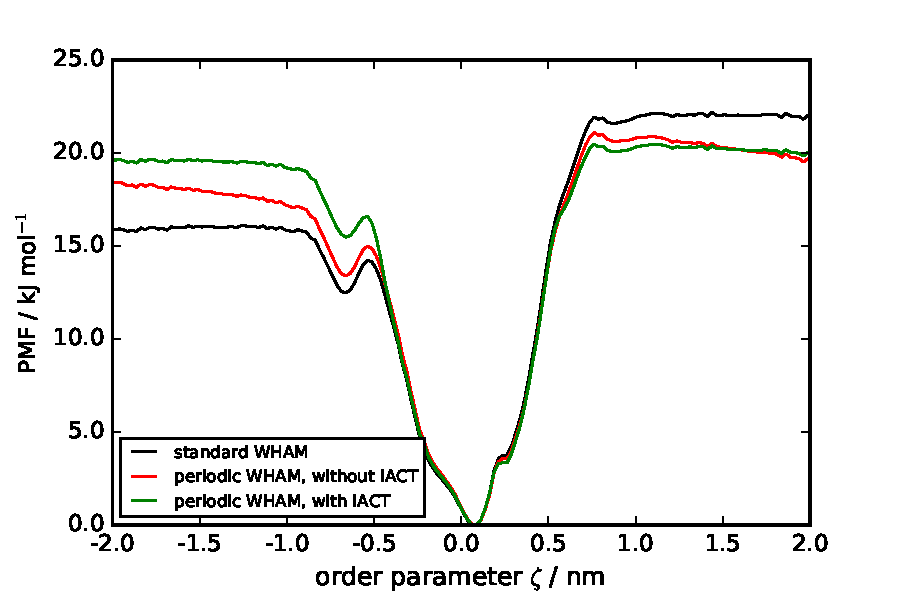
\includegraphics[width=\linewidth]{figures/pmf_aCD_BTL_gwham_cyclic.pdf}
  \caption{Effect of enforced periodicity (periodic) and integrated autocorrelation times (IACT) on the PMF estimation for the system 1-butanol / $\alpha$CD (Conf.~1).
  No orientational restraint was applied to the ligand.
  Calculation was performed using the \texttt{g\_wham} method~\cite{hub2010g_wham}. Error bars were neglected for clarity.
  Standard WHAM calculation (black curve) refers to estimation without IACT correction and without periodicity constraint.
  }
  \label{fig:gwham}
\end{figure}


\subsection{Influence of the Host's / Ligand's Flexibility}

If the host molecule is able to adopt multiple conformations, a bias might be introduced caused by the selection of initial conformations of the host or the method for generating starting configurations of the Umbrella windows. 
As found by You et al.~\cite{you2019potential}  
from studies of $\beta$CD complexes, significantly different PMF depths can be obtained depending on the initial host conformation unless simulation time was sufficient.
For such cases, discrepancies of the estimated binding free enthalpy compared to results from unbiased direct counting might be expected.
Due to the insensitivity of the adopted CNT conformations upon ligand binding alongside with the insensitivity of the PMFs towards increasingly restrictive restraining setups (c.f. Sec.~\ref{res:UnpMet_UnpCNT}),  
we do not expect such a bias in this case.
For further validation, a modified CNT was studied featuring decreased barriers for proper and improper dihedrals  compared to the standard model. 
Despite increased conformational flexibility, the resulting PMF obtained from the association with hexane (data not shown) was identical with the profile as shown in Fig.~\ref{fig:UU_MultiLig_CNT_electrst} (b).
For simulations based on  $\alpha$CD, we conclude from the good agreement between the PMF-based estimates for $\Delta G^\circ_\mathrm{bind}$ and the corresponding results from 
double decoupling~\cite{markthaler2017molecular, gebhardt2016calculation}
as well as direct counting~\cite{baz2018insights} that simulation time was sufficient in order to remove any possible bias due to the initial host conformations.
Moreover, the force field used in the present study does not show multiple conformations for $\alpha$CD~\cite{gebhardt2018validation}.
Considering host molecules which tend to undergo significant conformational changes upon ligand binding, the incorporation of a conformational restraint to bias the host conformation close to the bound state conformation might be advantageous~\cite{woo2005calculation}.
Moreover, the ligand conformation could be biased analogously which might be of practical value for speeding up convergence, especially for very flexible ligands.
The impact of such a conformational restraint with respect to the calculation of $\Delta G^\circ_\mathrm{bind}$ can be calculated rigorously~\cite{woo2005calculation}. 
In this case, Eq.~(\ref{eq:DG0_2}) has to be complemented by the free energy contribution from rigidification of the non-complexed host (unbound ligand) and 
the contribution from releasing the conformational restraint from the complexed host (bound ligand) again. 
To obtain accurate results for this process, the force field has to capture the relative energies of the different conformers very accurately~\cite{tirado2006contribution}.
As judged by the good agreement for the $\Delta G^\circ_\mathrm{bind}$ estimates obtained from the PMF and double decoupling in case of $\alpha$CD / dodecanol, 
we conclude that no conformational restraint is required for the flexible ligands considered in this work.


%%%%%%%%%%%%%%%%%%%%%%%%%%%%%%%%%%%%%%%%%%%%%%%%%%%%%%%%%%%%
\section{Conclusions}
%%%%%%%%%%%%%%%%%%%%%%%%%%%%%%%%%%%%%%%%%%%%%%%%%%%%%%%%%%%%

In this article, we studied the evaluation of one-dimensional potentials of mean force (PMF) of host-guest system obtained from Umbrella Sampling. 
A carbon nanotube (CNT) and $\alpha$-cyclodextrin ($\alpha$CD) were chosen as idealized model systems for pore- or channel-like protein host molecules featuring a hydrophobic cavity. 
A robust simulation protocol for the calculation of standard binding free enthalpies from such a PMF was established.
From systematic studies of different CNT / ligand combinations of increasing complexity, we could identify distinct computational artifacts that may occur in the PMF calculation.
Such artifacts which show up as PMF offset between the two flat bulk water regions prohibit an unambiguous estimation of the binding free enthalpy and have not been studied in detail so far.
It was found that despite an identical manifestation, three different origins for PMF offsets can be distinguished:
(i) an unfortunate choice of reference points for the Umbrella distance restraint;
(ii) a misfit in probability distributions between bound and unbound Umbrella windows in case of multiple binding modes; 
(iii) offsets introduced by the UI estimator due to non-Gaussian-shaped biased distribution functions.
It is important to distinguish these origins from possible primary reasons such as insufficient overlap between neighboring Umbrella windows (which is especially critical when estimation is performed with WHAM) 
or insufficient sampling time.
Neither the introduction of additional windows nor the extension of simulation time per window will eliminate the PMF artifacts in these cases.
It was shown that offsets due to (i) and (ii) can be eliminated by either restraining the ligand orientation close to the bound state orientation or through combination of the Umbrella Sampling setup with Replica Exchange (RE-US). 
Offsets resulting from the analysis method can be identified by comparing PMF results from different estimators (UI, MBAR, WHAM). 
Such a comparison which serves as consistency check is always recommended. 
We note that comparative simulations for $\alpha$CD / alcohol systems conducted with the CHARMM36 all-atom force field~\cite{markthaler2017molecular} also lead to PMF offsets if the ligand orientation was not restrained. 
This illustrates that the detected artifacts are force-field independent.
Regarding the influence of the simulation protocol, it can be expected that artifacts due to issues (i) and (ii) also 
occur for alternative PMF-based protocols such as Forward Flux Sampling if the ligand orientation is not preserved or proper sampling of multiple orientations can not be guaranteed.

%%%%%%%%%%%%%%%%%%%%%%%%%%%%%%%%%%%%%%%%%%%%%%%%%%%%%%%%%%%%
\section{Author Contributions}
%%%%%%%%%%%%%%%%%%%%%%%%%%%%%%%%%%%%%%%%%%%%%%%%%%%%%%%%%%%%
% This section must describe the actual contributions of
% author. Since this is an electronic-only journal, there is
% no length limit when you describe the authors' contributions,
% so we recommend describing what they actually did rather than
% simply categorizing them in a small number of
% predefined roles as might be done in other journals.
%
% See the policies ``Policies on Authorship'' section of https://livecoms.github.io
% for more information on deciding on authorship and author order.
%%%%%%%%%%%%%%%%

All authors designed the simulations, interpreted data and contributed to the writing of the paper. 
SJ and NH performed preliminary simulations leading to this project. DM carried out all simulations and analyses discussed in the manuscript.

% We suggest you preserve this comment:
%For a more detailed description of author contributions,
%see the GitHub issue tracking and changelog at \githubrepository.

%%%%%%%%%%%%%%%%%%%%%%%%%%%%%%%%%%%%%%%%%%%%%%%%%%%%%%%%%%%%
\section{Other Contributions}
%%%%%%%%%%%%%%%%%%%%%%%%%%%%%%%%%%%%%%%%%%%%%%%%%%%%%%%%%%%%
% You should include all people who have filed issues that were
% accepted into the paper, or that upon discussion altered what was in the paper.
% Multiple significant contributions might mean that the contributor
% should be moved to authorship at the discretion of the a
%
% See the policies ``Policies on Authorship'' section of https://livecoms.github.io for
% more information on deciding on authorship and author order.
%%%%%%%%%%%%%%%

The authors gratefully acknowledge Dr. Jens Kr\"uger for technical support as well as Prof. A. E. Mark and Prof. P. H. H\"unenberger for helpful discussion regarding the occurrence PMF offsets.
Moreover,  the authors thank  Prof. J. Pleiss from the University of Stuttgart who organized together with the author NH a seminar for the graduate school in Simulation Technology (GS SimTech)
during the winter semester 2014  which gave rise to fruitful discussions and inspiring ideas for the establishment of robust simulation protocols.
We thank Catharina Kleist and Felix Geisend\"orfer who, as students at the Hamburg University of Technology, performed some preliminary simulations for the present work.

%We suggest you preserve this comment:
%For a more detailed description of contributions from the community and others, see the GitHub issue tracking and changelog at \githubrepository.

%%%%%%%%%%%%%%%%%%%%%%%%%%%%%%%%%%%%%%%%%%%%%%%%%%%%%%%%%%%%
\section{Potentially Conflicting Interests}
%%%%%%%%%%%%%%%%%%%%%%%%%%%%%%%%%%%%%%%%%%%%%%%%%%%%%%%%%%%%

The authors declare no competing financial interest.

%%%%%%%%%%%%%%%%%%%%%%%%%%%%%%%%%%%%%%%%%%%%%%%%%%%%%%%%%%%%
\section{Funding Information}
%%%%%%%%%%%%%%%%%%%%%%%%%%%%%%%%%%%%%%%%%%%%%%%%%%%%%%%%%%%%
% Authors should acknowledge funding sources here. Reference specific grants.
%%%%%%%
This work was financially supported by the Ministry of Science, Research and Arts and the Universities of the State of Baden-W\"urttemberg, Germany and the German Research Foundation (DFG) 
through the collaborative research center SFB 716 and the Cluster of Excellence in Simulation Technology (EXC 310/2), both at the University of Stuttgart. 
Simulations were performed on the computational facility BinAC funded by the Ministry of Science, Research and Arts and the Universities of the State of Baden-W\"urttemberg, Germany within 
the framework program bwHPC and the DFG through grant no. INST 39/9631 FUGG.
SJ thanks the North-German Supercomputing Alliance (HLRN) for providing computational resources.

%%%%%%%%%%%%%%%%%%%%%%%%%%%%%%%%%%%%%%%%%%%%%%%%%%%%%%%%%%%%
\section*{Author Information}
%%%%%%%%%%%%%%%%%%%%%%%%%%%%%%%%%%%%%%%%%%%%%%%%%%%%%%%%%%%%
\makeorcid

\nocite{*} % This command displays all refs in the bib file
\bibliography{references}

%%%%%%%%%%%%%%%%%%%%%%%%%%%%%%%%%%%%%%%%%%%%%%%%%%%%%%%%%%%%
%%% APPENDICES
%%%%%%%%%%%%%%%%%%%%%%%%%%%%%%%%%%%%%%%%%%%%%%%%%%%%%%%%%%%%
%\clearpage

\appendix
\setcounter{table}{0}
\renewcommand{\thetable}{A\arabic{table}}


\section*{Appendix}

\subsection*{Double Decoupling}

According to the double decoupling method (DDM), 
the calculation of the standard binding free enthalpy reads as~\cite{deng2009computations}:
\begin{equation}
\Delta G^\circ_\mathrm{bind} = \Delta G^\mathrm{L \rightarrow D}_\mathrm{u} - \Delta G^\mathrm{L}_\mathrm{b, 0 \rightarrow R} - \Delta G^\mathrm{L \rightarrow D}_\mathrm{b, R} 
- \Delta G^\mathrm{D}_\mathrm{b, R \rightarrow 0} 
\label{eq:DG0_DDM}
\end{equation}
$\Delta G^\mathrm{L \rightarrow D}_\mathrm{u}$ refers to the free energy contribution for transforming the fully interacting unbound ligand (L) into its ideal gas or decoupled (D) state. 
%It corresponds to the negative hydration free enthalpy.
$\Delta G^\mathrm{L \rightarrow D}_\mathrm{b, R}$ represents the analogue contribution for the ligand bound to the CNT host.
To prevent drifting of the decoupled ligand, an auxiliary translational (and possibly orientational) restraint (R) has to be applied.
The translational and orientational restraints were implemented as harmonic potentials acting on the host-ligand COM-COM radial distance and the orientational angle $\theta$, respectively. 
$\Delta G^\mathrm{L}_\mathrm{b, 0 \rightarrow R}$ and $\Delta G^\mathrm{D}_\mathrm{b, R \rightarrow 0}$ refer to the contributions due to application and release of the auxiliary restraints 
for the fully interacting and decoupled ligand in the bound state, respectively.
Decoupling of the ligand from the bulk solvent and host was conducted in a sequence of 20 discrete steps as controlled by the coupling parameter $\lambda$, equally  distributed between $\lambda = 0$ (fully interacting) 
and $\lambda = 1$ (decoupled state).
It should be stressed that since DDM was applied for systems unpolar CNT / unpolar ligand, the scaling with $\lambda$ solely affects the dispersion interactions with the environment.
Activation of the translational %(and orientational) 
restraint in case of the fully interacting bound ligand was performed in 11 distinct simulations using uniformly increasing values for the force constant between 0 and 
500 kJ~mol$^{-1}$~nm$^{-2}$. 
In case of an additional orientational restraint, it was activated simultaneously with the translational restraint using uniformly increasing values for the force constant between 0 and 500 kJ~mol$^{-1}$~rad$^{-2}$.
The MBAR free energy estimator was used in all cases.
The contribution $\Delta G^\mathrm{D}_\mathrm{b, R \rightarrow 0}$ was calculated analytically according to~\cite{hermans1997inclusion}:
\begin{equation}
\Delta G^\mathrm{D}_\mathrm{b, R \rightarrow 0} =  - RT \ln \left(\frac{V^\circ \, 8 \pi^2}{V_\mathrm{tr} \, \Omega} \right) 
\label{eq:DGrottrans_DDM}
\end{equation}
%
with the accessible translational and rotational volumes of
\begin{eqnarray}
V_\mathrm{tr} & = & \left( \frac{2 \pi RT}{k_\mathrm{tr}}\right)^\frac{3}{2} \\
\frac{\Omega}{8 \pi^2} & = & \frac{1}{2} \int\limits_{0}^{\pi} \mathrm{e}^{- U_\theta(\theta)/RT} \, \sin\theta \, \mathrm{d}\theta
\end{eqnarray}


In case of a harmonic potential $U_\theta(\theta)$ according to Eq.~(\ref{eq:ori_restr}), the rotational volume $V_\mathrm{rot}$ was calculated numerically while it reduces to unity in the absence of an orientational restraint. 
Calculated binding free enthalpies from DDM for systems unpolar ligand / unpolar CNT are summarized in Tab.~\ref{tbl:DDM}. 
In all simulations, long-range electrostatics were treated with  the particle-mesh Ewald (PME) method.

\begin{table*}[htb!]
\caption{\label{tbl:DDM} 
Calculated standard binding free enthalpies $\Delta G^\circ_\mathrm{bind}$ from  double decoupling for unpolar methane, ethane and elongated ethane binding to unpolar CNT.
The two ethane models contain two rows of data, corresponding to the setup with and without orientational restraint (OR).
Detailed description of the double decoupling approach can be found in the appendix.
$\Delta G^\mathrm{L \rightarrow D}_\mathrm{u}$, $\Delta G^\mathrm{L \rightarrow D}_\mathrm{b, R}$ and $\Delta G^\mathrm{L}_\mathrm{b, 0 \rightarrow R}$ were calculated using the MBAR estimator.
The contribution for removing the restraints from the decoupled ligand ($\Delta G^\mathrm{D}_\mathrm{b, R \rightarrow 0}$) was calculated analytically according to Eq.~(\ref{eq:DGrottrans_DDM}).
The estimate of $\Delta G^\circ_\mathrm{bind, Conf. 1}$ as obtained from the setup including an orientational restraint corresponds to one distinct binding configuration and has to be corrected 
by an entropic symmetry term of $-RT \ln 2$~\cite{gilson2013correction, hermans1997inclusion} to obtain $\Delta G^\circ_\mathrm{bind}$ in case of elongated ethane.
Estimates for statistical uncertainties of $\Delta G^\circ_\mathrm{bind}$ as obtained from application of standard error propagation to Eq.~\ref{eq:DG0_DDM} are below 0.5~kJ~mol$^{-1}$ where 
the statistical uncertainties of the individual free energy terms are delivered by the MBAR estimator~\cite{shirts2008statistically}.
}
\centering
\begin{tabular}{llc ccc cc}\hline
System & Setup & $\Delta G^\mathrm{L \rightarrow D}_\mathrm{u}$ & $\Delta G^\mathrm{L \rightarrow D}_\mathrm{b, R}$ & $\Delta G^\mathrm{L}_\mathrm{b, 0 \rightarrow R}$ & 
$\Delta G^\mathrm{D}_\mathrm{b, R \rightarrow 0}$ & $\Delta G^\circ_\mathrm{bind, Conf. 1}$ & $\Delta G^\circ_\mathrm{bind}$ \\
& & $[\mathrm{kJ~mol}^{-1}]$ & $[\mathrm{kJ~mol}^{-1}]$ & $[\mathrm{kJ~mol}^{-1}]$ & $[\mathrm{kJ~mol}^{-1}]$ & $[\mathrm{kJ~mol}^{-1}]$ & $[\mathrm{kJ~mol}^{-1}]$ \\ 
\hline
Methane 						& & -9.60	& 13.78	& 3.86 & -14.22 & - & -13.00 \\
\hline
\multirow{ 2}{*}{Ethane}  	& No OR & -7.37 & 30.82 & 2.38 & -14.22 & - & -26.35 \\
					& OR       & -7.37 & 31.99 & 17.03 & -29.15 & -27.23 & -27.23 \\
\hline
\multirow{ 2}{*}{Long Ethane}  & No OR & -22.67 & 14.32 & 2.32 & -14.22 & - & -25.09\\  
					      & OR       & -22.67 & 22.23 & 8.31 & -29.15 & -24.06 & -25.79\\
\hline
\end{tabular}
\end{table*}


\end{document}